\documentclass[12pt]{thesul}
%----------------------------------------------------------------------
%                               Packages
%----------------------------------------------------------------------
\usepackage[french]{babel}
\usepackage{acronym} % \ac[p], \acl[p], \acs[p], \acf[p]
\usepackage[maxbibnames=99,maxcitenames=1,sorting=none]{biblatex}
\bibliography{biblio.bib}
\usepackage{booktabs} % \toprule, \midrule, \cmidrule, \bottomrule
\usepackage{cancel} % \cancel
\usepackage{caption}
\usepackage{csquotes}
\usepackage{hyperref}
\hypersetup{hidelinks}
\usepackage[inline]{enumitem}
\setlist[enumerate]{label=(\roman*)} %% <- set the base level label separately
\usepackage{import} % \import
\usepackage[french]{minitoc}

\usepackage{xcolor}
\AtBeginDocument{
\definecolor{lfsgreen}{RGB}{31,160,31}
\definecolor{lfsorange}{RGB}{255,178,2}
\definecolor{lfsred}{RGB}{160,30,31}

% white
\definecolor{uclwhite}{rgb}{1, 1, 1}

%   UCL style guide colours.
%   Number refer to level of tint.
%   100%    1
%    70%    2
%    50%    3
%    20%    4

 % UCL style guide dk purple
\definecolor{ucl1dkpurple}{RGB}{82,66,91}
\definecolor{ucl2dkpurple}{RGB}{134,122,140}
\definecolor{ucl3dkpurple}{RGB}{168,160,173}
\definecolor{ucl4dkpurple}{RGB}{220,217,222}

 % UCL style guide dk red
\definecolor{ucl1dkred}{RGB}{90,27,49}
\definecolor{ucl2dkred}{RGB}{139,95,110}
\definecolor{ucl3dkred}{RGB}{172,141,152}
\definecolor{ucl4dkred}{RGB}{222,209,214}

 % UCL style guide dk blue
\definecolor{ucl1dkblue}{RGB}{0,67,89}
\definecolor{ucl2dkblue}{RGB}{76,123,138}
\definecolor{ucl3dkblue}{RGB}{127,161,172}
\definecolor{ucl4dkblue}{RGB}{204,217,222}

 % UCL style guide dk green
\definecolor{ucl1dkgreen}{RGB}{75,70,32}
\definecolor{ucl2dkgreen}{RGB}{129,125,98}
\definecolor{ucl3dkgreen}{RGB}{165,162,143}
\definecolor{ucl4dkgreen}{RGB}{219,218,210}

 % UCL style guide black
\definecolor{ucl1black}{RGB}{0,0,0}
\definecolor{ucl2black}{RGB}{75,75,75}
\definecolor{ucl3black}{RGB}{128,128,128}
\definecolor{ucl4black}{RGB}{205,205,205}

 % UCL style guide pink
\definecolor{ucl1pink}{RGB}{145,24,83}
\definecolor{ucl2pink}{RGB}{178,93,134}
\definecolor{ucl3pink}{RGB}{200,139,169}
\definecolor{ucl4pink}{RGB}{233,209,221}

 % UCL style guide md red
\definecolor{ucl1mdred}{RGB}{195,58,45}
\definecolor{ucl2mdred}{RGB}{213,117,108}
\definecolor{ucl3mdred}{RGB}{225,156,150}
\definecolor{ucl4mdred}{RGB}{243,216,213}

 % UCL style guide md blue
\definecolor{ucl1mdblue}{RGB}{69,156,189}
\definecolor{ucl2mdblue}{RGB}{124,186,209}
\definecolor{ucl3mdblue}{RGB}{162,205,222}
\definecolor{ucl4mdblue}{RGB}{218,235,242}

 % UCL style guide md green
\definecolor{ucl1mdgreen}{RGB}{130,141,55}
\definecolor{ucl2mdgreen}{RGB}{167,175,115}
\definecolor{ucl3mdgreen}{RGB}{192,198,155}
\definecolor{ucl4mdgreen}{RGB}{230,232,215}

 % UCL style guide orange
\definecolor{ucl1orange}{RGB}{215,123,35}
\definecolor{ucl2orange}{RGB}{227,162,101}
\definecolor{ucl3orange}{RGB}{235,189,145}
\definecolor{ucl4orange}{RGB}{247,229,211}

  % UCL style guide lt purple
\definecolor{ucl1ltpurple}{RGB}{191,175,188}
\definecolor{ucl2ltpurple}{RGB}{210,199,208}
\definecolor{ucl3ltpurple}{RGB}{223,215,221}
\definecolor{ucl4ltpurple}{RGB}{242,239,242}

 % UCL style guide yellow
\definecolor{ucl1yellow}{RGB}{229,175,0}
\definecolor{ucl2yellow}{RGB}{237,199,76}
\definecolor{ucl3yellow}{RGB}{242,215,127}
\definecolor{ucl4yellow}{RGB}{250,239,204}

 % UCL style guide lt blue
\definecolor{ucl1ltblue}{RGB}{168,192,209}
\definecolor{ucl2ltblue}{RGB}{194,211,223}
\definecolor{ucl3ltblue}{RGB}{211,223,232}
\definecolor{ucl4ltblue}{RGB}{238,242,246}

% UCL style guide brt green
\definecolor{ucl1brtgreen}{RGB}{204,209,88}
\definecolor{ucl2brtgreen}{RGB}{219,223,138}
\definecolor{ucl3brtgreen}{RGB}{229,232,171}
\definecolor{ucl4brtgreen}{RGB}{245,246,222}

% UCL style guide stone
\definecolor{ucl1stone}{RGB}{217,214,204}
\definecolor{ucl2stone}{RGB}{228,226,219}
\definecolor{ucl3stone}{RGB}{236,234,229}
\definecolor{ucl4stone}{RGB}{255,255,255}

% UCL style guide lt green
\definecolor{ucl1ltgreen}{RGB}{185,193,147}
\definecolor{ucl2ltgreen}{RGB}{206,211,179}
\definecolor{ucl3ltgreen}{RGB}{220,224,201}
\definecolor{ucl4ltgreen}{RGB}{241,243,233}

\definecolor{darkgreen}{RGB}{75,70,32}
\definecolor{darkblue}{RGB}{0,67,89}
\definecolor{mydarkblue}{RGB}{76,123,138}
\definecolor{mydarkblueid}{RGB}{0,67,89}
\definecolor{mylightblue}{RGB}{168,192,209}
\definecolor{mydarkorange}{RGB}{215,123,35}
\definecolor{mylightorange}{RGB}{227,162,101}
\definecolor{mydarkred}{RGB}{90,27,49}
\definecolor{mydarkpurple}{RGB}{134,122,140}
\definecolor{mydarkpurpleid}{RGB}{82,66,91}
}

\usepackage{amssymb}
\usepackage{amsmath}
\usepackage{amsthm}
% \interdisplaylinepenalty=2500
\theoremstyle{definition}
\newtheorem{definition}{Définition}
\newtheorem{subdefinition}{Définition}[definition]
\newtheorem{myrule}{Règle}
\newtheorem{property}{Propriété}
\newtheorem{subproperty}{Propriété}[property]
\usepackage{MnSymbol} % \dashrightarrow

\usepackage{algorithm, algpseudocode}
\floatname{algorithm}{Algorithme} % Renomme caption de "Algorithm" -> "Algorithme"

\newcommand\CONDITION[2]%
  {\begin{tabular}[t]{@{}l@{}l@{}}
     #1&#2
   \end{tabular}%
  }
  \algdef{SE}[WHILE]{While}{EndWhile}[1]%
  {\algorithmicwhile\ \CONDITION{#1}{\ \algorithmicdo}}%
  {\algorithmicend\ \algorithmicwhile}
\algdef{SE}[FOR]{For}{EndFor}[1]%
  {\algorithmicfor\ \CONDITION{#1}{\ \algorithmicdo}}%
  {\algorithmicend\ \algorithmicfor}
\algdef{S}[FOR]{ForAll}[1]%
  {\algorithmicforall\ \CONDITION{#1}{\ \algorithmicdo}}
\algdef{SE}[REPEAT]{Repeat}{Until}{\algorithmicrepeat}[1]%
  {\algorithmicuntil\ \CONDITION{#1}{}}
\algdef{SE}[IF]{If}{EndIf}[1]%
  {\algorithmicif\ \CONDITION{#1}{\ \algorithmicthen}}%
  {\algorithmicend\ \algorithmicif}%
\algdef{C}[IF]{IF}{ElsIf}[1]%
  {\algorithmicelse\ \algorithmicif\ \CONDITION{#1}{\ \algorithmicthen}}

\usepackage[inline,nomargin,index]{fixme}
\fxsetup{theme=color,mode=multiuser,inlineface=\itshape,envface=\itshape}
\FXRegisterAuthor{mn}{amn}{Matthieu}

\usepackage{tikz} % \begin{tikzpicture} \end{tikzpicture}
\usetikzlibrary{calc}
\usetikzlibrary{graphs}
\usetikzlibrary{quotes}
\usetikzlibrary{shapes.misc}

\usepackage[caption=false,font=footnotesize,labelfont=sf,textfont=sf]{subfig}

\usepackage{marvosym} % \Flatsteel
\usepackage{wasysym} % \checked

\usepackage{pifont} % \ding
\renewcommand{\checkmark}{\ding{51}}
\newcommand{\ballotx}{\ding{55}}

\usepackage{xspace} % \xspace

% Commands
%---------
\newcommand{\cf}[1]{(cf. \autoref{#1}, page \pageref{#1})}
\newcommand{\eg}{e.g.\xspace}
\newcommand{\ie}{c.-à-d.\xspace}

\newcommand{\hb}{\emph{happens-before}\xspace}

\newcommand{\inbb}[1]{\in \mathbb{#1}}
\newcommand{\new}{\textbf{new}}
\newcommand{\trm}[1]{\mathit{#1}}
\newcommand{\set}[1]{\left\{#1\right\}} % set brace notation

\newcommand{\betterid}[3]{\trm{#1}^{\trm{#2}}_{\trm{#3}}}
\newcommand{\id}[3]{$\trm{#1}^{\trm{#2}}_{\trm{#3}}$}
\newcommand{\epoch}[1]{$\varepsilon_{#1}$}
\newcommand{\lid}{<_{id}}
\newcommand{\leqid}{$\leq_{id}$~}
\newcommand{\lepoch}{$<_{\varepsilon}$~}
\newcommand{\leqepoch}{$\leq_{\varepsilon}$~}
\newcommand{\ltuple}{<_{t}}

\newcommand{\botn}{\bot_\mathbb{N}}
\newcommand{\topn}{\top_\mathbb{N}}
\newcommand{\logootuple}[1]{\langle \text{pos}_{#1},\text{nodeId}_{#1},\text{seq}_{#1} \rangle}

\newcommand{\bigO}[1]{$\mathcal{O}(#1)$}

\newcommand{\widthletter}{2em}
\newcommand{\widthblock}{3em}
\newcommand{\widthoriginepoch}{1.33em}
\newcommand{\widthepoch}{1.65em}

\newcommand{\withmathbreak}[1]{\parbox{\linewidth}{#1}}
\newcommand{\elt}{E}
\newcommand{\nat}{\mathbb{N}}


% Définit noms pour \autoref
%---------
\newcommand{\algorithmautorefname}{Algorithme}
\newcommand{\annexautorefname}{Annexe}
\newcommand{\definitionautorefname}{Définition}
\newcommand{\propertyautorefname}{Propriété}
\newcommand{\subfigureautorefname}{Figure}
\newcommand{\subpropertyautorefname}{Propriété}

% Tikz styles
\tikzset{
    common/.style={anchor=west, draw, rectangle, minimum height=6mm},
    letter/.style={common, minimum width=\widthletter},
    block/.style={common, minimum width=\widthblock},
    epoch/.style={letter, rounded rectangle, rounded rectangle east arc=0pt, minimum width=\widthepoch},
    point/.style={insert path={ node[scale=5*sqrt(\pgflinewidth)]{.} }},
    node/.style={draw, circle, minimum size=1em},
    op/.style={draw, circle, minimum size=2.7em},
    causalop/.style={op, double=white, inner sep=2pt},
    gc-rule-1/.style={dashed, thick, darkblue},
    gc-rule-2/.style={densely dotted, thick, darkgreen},
    cross/.style={
        path picture={
            \draw[ucl1dkred, very thick]
                (path picture bounding box.south east)--(path picture bounding box.north west)
                (path picture bounding box.south west)--(path picture bounding box.north east);
        }
    }
}


%-------------------------------------------------------------------
%                             Marges
%-------------------------------------------------------------------

% pour positionner les vraies marges:
%\SetRealMargins{1mm}{1mm}

%-------------------------------------------------------------------
%                             En-têtes
%-------------------------------------------------------------------

% Les en-têtes: quelques exemples
%\UppercaseHeadings
%\UnderlineHeadings
%\newcommand\bfheadings[1]{{\bf #1}}
%\FormatHeadingsWith{\bfheadings}
%\FormatHeadingsWith{\uppercase}
%\FormatHeadingsWith{\underline}
\newcommand\upun[1]{\uppercase{\underline{\underline{#1}}}}
\FormatHeadingsWith\upun

\newcommand\itheadings[1]{\textit{#1}}
\FormatHeadingsWith{\itheadings}

% pour avoir un trait sous l'en-tete:
\setlength{\HeadRuleWidth}{0.4pt}

%-------------------------------------------------------------------
%                         Les références
%-------------------------------------------------------------------

\NoChapterNumberInRef
\NoChapterPrefix

%-------------------------------------------------------------------
%                           Brouillons
%-------------------------------------------------------------------

% ceci ajoute une marque « brouillon » et la date
\ThesisDraft

%-------------------------------------------------------------------
%                   Pour collecter un glossaire et un index
%-------------------------------------------------------------------

\makeglossary
\makeindex

%-------------------------------------------------------------------
%                           Acronymes
%-------------------------------------------------------------------

% Acronyms
% --------
% \input{assets/acronyms.tex}
\acrodef{ADT}[ADT]{Abstract Data Type}
\acrodefplural{ADT}[ADTs]{Abstract Data Types}
\acrodef{API}[API]{Application Programming Interface}
\acrodef{AW}[AW]{\emph{Add-Wins}}
\acrodef{CCI}[CCI]{Convergence, Causality preservation, Intention preservation}
\acrodef{CL}[CL]{\emph{Causal-Length}}
\acrodef{CRDT}[CRDT]{Conflict-free Replicated Data Type}
\acrodefplural{CRDT}[CRDTs]{Conflict-free Replicated Data Types}
\acrodef{DAG}[DAG]{Directed Acyclic Graph}
\acrodef{FIFO}[FIFO]{First In, First Out}
\acrodef{GC}[GC]{Garbage Collection}
\acrodef{IPFS}[IPFS]{InterPlanetary File System}
\acrodef{JIT}[JIT]{Just-In-Time}
\acrodef{LCA}[PPAC]{Plus Petit Ancêtre Commun}
\acrodef{LFS}[LFS]{Local-First Software}
\acrodefplural{LFS}[LFS]{Local-First Softwares}
\acrodef{LUB}[LUB]{Least Upper Bound}
\acrodef{LWW}[LWW]{\emph{Last-Writer-Wins}}
\acrodef{MUTE}[MUTE]{Multi User Text Editor}
\acrodef{MV}[MV]{\emph{Multi-Value}}
\acrodef{OC}[OC]{Commutativité des Opérations}
\acrodef{OT}[OT]{Operational Transformation}
\acrodefplural{OT}[OT]{Operational Transformations}
\acrodef{P2P}[P2P]{Pair-à-Pair}
\acrodef{PKI}[PKI]{Public Key Infrastructure}
\acrodef{PoC}[PoC]{Proof of Concept}
\acrodef{PT}[PT]{Transitivité de la Précédence}
\acrodef{RADT}[RADT]{Replicated Abstract Data Type}
\acrodefplural{RADT}[RADTs]{Replicated Abstract Data Types}
\acrodef{RCB}[RCB]{Reliable Causal Broadcast}
\acrodef{RGA}[RGA]{Replicated Growable Array}
\acrodef{RW}[RW]{\emph{Remove-Wins}}
\acrodef{SEC}[SEC]{Cohérence forte à terme}
\acrodef{TTF}[TTF]{Tombstone Transformation Function}
\acrodefplural{TTF}[TTF]{Tombstone Transformation Functions}
\acrodef{WebRTC}[WebRTC]{Web Real-Time Communication}

%-------------------------------------------------------------------
%                           Couleurs
%-------------------------------------------------------------------

% \input{assets/colours.tex}

%-------------------------------------------------------------------
%                     Global custom tikz commands
%-------------------------------------------------------------------

% \input{assets/tikz_presets.tex}

\begin{document}


      \OddHead={{\leftmark\rightmark}{\hfil\slshape\rightmark}}
      \EvenHead={{\leftmark}{{\slshape\leftmark}\hfil}}
      \OddFoot={\hfil\thepage}
      \EvenFoot={\thepage\hfil}
      \pagestyle{ThesisHeadingsII}


%-------------------------------------------------------------------
%                          Encadrements
%-------------------------------------------------------------------

% encadre les chapitres dans la table des matières:
% (ces commandes doivent figurer apres \begin{document}

\FrameChaptersInToc
%\FramePartsInToc


%-------------------------------------------------------------------
%            Réinitialisation de la numérotation des chapitres
%-------------------------------------------------------------------

% Si la commande suivante est présente,
% elle doit figurer APRÈS \begin{document}
% et avant la première commande \part
\ResetChaptersAtParts

%-------------------------------------------------------------------
%               mini-tables des matières par chapitre
%-------------------------------------------------------------------

% préparer les mini-tables des matières par chapitre.
% (commande de minitoc.sty)
\dominitoc

%-------------------------------------------------------------------
%                         Page de titre:
%-------------------------------------------------------------------

\ThesisTitle{Ré-identification sans coordination dans les types de données répliquées sans conflits (CRDTs)}
\ThesisDate{TODO: Définir une date}
\ThesisAuthor{Matthieu Nicolas}

% Type de la these
\ThesisUL
% Jury:

% (ne pas mettre de \\ apres la dernière entree)

% Exemple de création d'une nouvelle catégorie dans le jury:

% \NewJuryCategory{Encadrants}{\it Encadrant :}
%                        {\it Encadrants :}

\def\blanc{\hspace*{1cm}}

\President    = {À déterminer}
\Rapporteurs  = {Hanifa Boucheneb & Professeure, Polytechnique Montréal\\
                 Davide Frey      & Chargé de recherche, HdR, Inria Rennes Bretagne-Atlantique}
\Examinateurs = {Hala Skaf-Molli  & Maîtresse de conférences, HdR, Nantes Université \\
                 Stephan Merz     & Directeur de Recherche, Inria Nancy - Grand Est}
\Encadrants= {Olivier Perrin      & Professeur des Universités, Université de Lorraine, LORIA \\
              Gérald Oster        & Maître de conférences, Université de Lorraine, LORIA}

%\Invites=       {}

% Création de la page de titre:
\MakeThesisTitlePage

%-------------------------------------------------------------------


%-------------------------------------------------------------------
%                          remerciements
%-------------------------------------------------------------------

%\DontFrameThisInToc
\begin{ThesisAcknowledgments}
WIP
\end{ThesisAcknowledgments}

%-------------------------------------------------------------------
%                            dédicace
%-------------------------------------------------------------------

\begin{ThesisDedication}
WIP
\end{ThesisDedication}


%-------------------------------------------------------------------
%                  écriture de `Chapitre' et `Partie'
%                      dans la table des matières
%-------------------------------------------------------------------

\WritePartLabelInToc
\WriteChapterLabelInToc

%-------------------------------------------------------------------
%                        table des matières
%-------------------------------------------------------------------

\tableofcontents

%-------------------------------------------------------------------
%              Exemple d'utilisation de \SpecialSection
%-------------------------------------------------------------------
%\SpecialSection{Introduction générale}

\DontWriteThisInToc
\listoffigures

\mainmatter
\NumberThisInToc
\chapter{Introduction}
\minitoc

\section{Contexte}
\label{sec:intro-contexte}

L'évolution des technologies du web a conduit à l'avènement de ce qui est communément appelé le Web 2.0.
La principale caractéristique de ce média est la possibilité aux utilisateur-rices non plus seulement de le consulter, mais aussi d'y contribuer.

Ces nouvelles fonctionnalités ont permis l'apparition d'applications incitant les utilisateur-rices à créer et partager leur propre contenu, ainsi que d'échanger avec d'autres utilisateur-rices à ce sujet.
Un cas particulier de ces applications proposent aux utilisateur-rices de travailler ensemble pour la création d'un même contenu, en d'autres termes de collaborer.
Nous appelons ces applications des \emph{systèmes collaboratifs} :
\begin{definition}[Système collaboratif]
  \label{def:collaborative-system}
  Un système collaboratif est un système supportant ses utilisateur-rices dans leurs processus de collaboration pour la réalisation de tâches.
\end{definition}

De nos jours, ces systèmes font parties des applications les plus populaires du paysage internet, \eg GoogleDocs compte XX millions utilisateur-rices, GitHub YY millions, Wikipedia 788 millions {\cite{2022-09-monthly-active-users-wikipedia}} ou Quora 300 millions \cite{2022-01-monthly-active-users-social-networks}.
\mnnote{TODO: Ajouter chiffres et refs}
De leur côté, d'autres plateformes impliquent leur communautés en organisant ponctuellement des collaborations éphémères et généralement massives, \eg r/Place \cite{2022-rplace} ou TwitchPlaysPokemon \cite{2014-twitch-plays-pokemon}.\\

En raison de leur popularité, les systèmes collaboratifs doivent assurer plusieurs propriétés pour garantir leur bon fonctionnement et qualité de service : une haute disponibilité, tolérance aux pannes et capacité de passage à l'échelle.
\begin{definition}[Disponibilité]
  \label{def:availability}
  La disponibilité d'un système indique sa capacité à répondre à tout moment à une requête d'un-e utilisateur-rice.
\end{definition}
\begin{definition}[Tolérance aux pannes]
  La tolérance aux pannes d'un système indique sa capacité à continuer à répondre aux requêtes malgré l'absence de réponse d'un ou plusieurs de ses composants.
\end{definition}
\begin{definition}[Capacité de passage à l'échelle]
  La capacité de passage à l'échelle d'un système indique sa capacité à traiter un volume toujours plus conséquent de requêtes.
\end{definition}

Pour cela, ces systèmes adoptent une architecture décentralisée, que nous illustrons par la \autoref{fig:decentralised-system}.
\begin{figure}[!ht]
  \centering
  \resizebox{0.3 \columnwidth}{!}{
    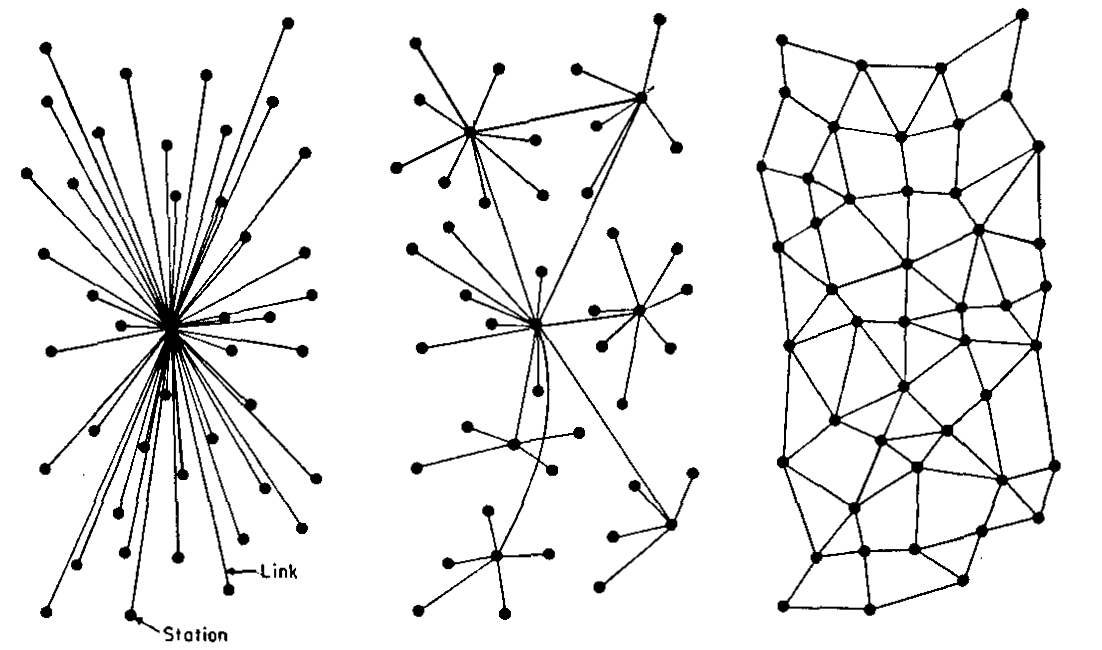
\includegraphics[trim=12cm 0cm 13cm 0cm, clip]{img/centralised-decentralised-distributed}
  }
  \caption[Caption for decentralised-system]{Représentation d'une architecture décentralisée\footnotemark}
  \label{fig:decentralised-system}
\end{figure}
\footnotetext{Source : \cite{1964-distributed-communications-networks-baran}}

Dans ce type d'architecture, les responsabilités, tâches et la charge travail sont réparties entre un ensemble de serveurs.
Il convient toutefois de noter que les serveurs jouent de manière globale toujours un rôle central dans ces systèmes, malgré ce que le nom de cette architecture peut suggérer.
En effet, ces systèmes reposent toujours sur leurs serveurs pour authentifier les utilisateur-rices, stocker les données de leurs utilisateur-rices ou encore fusionner les modifications effectuées par ces dernier-es.\\
% La nuance porte seulement sur le fait que ce n'est plus un serveur unique qui est en charge de ces tâches, mais un ensemble de serveurs.

Bien que cette architecture système permette de répondre aux problèmes d'ordre technique que nous présentons précédemment, nous considérons que cette architecture souffre néanmoins de limites.
Notamment, de part le rôle prédominant que jouent les serveurs dans les systèmes décentralisés, ces derniers échouent à assurer un second ensemble de propriétés, que nous jugeons néanmoins fondamentales :
\begin{definition}[Confidentialité des données]
  \label{def:confidentialite}
  La confidentialité des données d'un système indique sa capacité à garantir à ses utilisateur-rices que leurs données ne seront pas accessibles par des tiers non autorisés ou par le système lui-même.
\end{definition}
\begin{definition}[Souveraineté des données]
  \label{def:souverainete}
  La souveraineté des données d'un système indique sa capacité à garantir à ses utilisateur-rices leur maîtrise de leurs données, \ie leur capacité à les consulter, modifier, partager, exporter; supprimer ou encore à décider de l'usage qui en est fait.
\end{definition}
\begin{definition}[Pérennité]
  \label{def:perennite}
  La pérennité d'un système indique sa capacité à garantir à ses utilisateur-rices son fonctionnement continu dans le temps.
\end{definition}
\begin{definition}[Résistance à la censure]
  \label{def:censorship}
  La résistance à la censure d'un système indique sa capacité à garantir à ses utilisateur-rices son fonctionnement malgré des actions de contrôle de l'information par des autorités.
\end{definition}

De plus, les serveurs ne sont pas une ressource libre.
En effet, ils sont déployés et maintenus par la ou les organisations qui proposent le système collaboratif.
Ces organisations font alors office d'\emph{autorités centrales} du système, \eg en se portant garantes de l'identité des utilisateur-rices, de l'authenticité d'un contenu ou encore de la disponibilité dudit contenu.

De part le fait que les autorités centrales possèdent les serveurs hébergeant le système, elles ont tout pouvoir sur ces derniers.
Ainsi, les utilisateur-rices de systèmes collaboratifs prennent, de manière consciente ou non, le risque que les propriétés présentées précédemment soient transgressées par les autorités auxquelles appartiennent ces applications ou par des tiers avec lesquelles ces autorités interagissent, \eg des gouvernements.
Plusieurs faits d'actualités nous ont malheureusement montré de tels faits, \eg la censure de Wikipedia par des gouvernements \cite{2022-wikipedia-censorship}, la fermeture de services par les entreprises les proposant \cite{2022-killed-by-google} ou encore la mise à disposition des données hébergées par les GAFAMs aux services de renseignement de différentes nations \cite{prism-guardian,prism-washington-post}.
Cependant, le coût de l'infrastructure nécessaire pour déployer des systèmes à large échelle équivalents entrave l'apparition d'alternatives, plus respectueuses de leurs utilisateur-rices.\\

\emph{Ainsi, il nous paraît fondamental de proposer des moyens technologiques rendant accessible la conception et le déploiement des systèmes collaboratifs alternatifs.
Ces derniers devraient minimiser le rôle des autorités centrales, voire l'éliminer, de façon à protéger les intérêts de leurs utilisateur-rices.}\\

Dans cette optique, une piste de recherche que nous jugeons intéressante à étudier est celle des systèmes collaboratifs \acf{P2P}.
Cette architecture système, que nous illustrons par la \autoref{fig:distributed-system}, place les utilisateur-rices au centre du système et relègue les éventuels serveurs à un simple rôle de support de la collaboration, \eg la mise en relation des pairs.

\begin{figure}[!ht]
  \centering
  \resizebox{0.25 \columnwidth}{!}{
    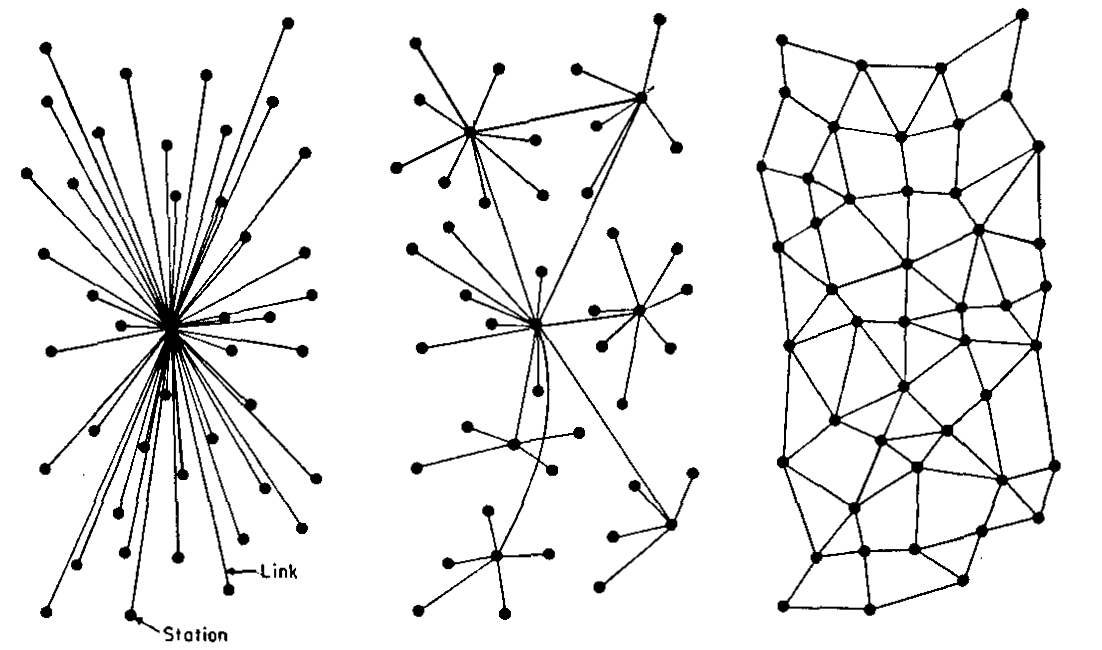
\includegraphics[trim=26cm 0cm 1cm 0cm, clip]{img/centralised-decentralised-distributed}
  }
  \caption[Caption for distributed-system]{Représentation d'une architecture distribuée\footnotemark[\value{footnote}]}
  \label{fig:distributed-system}
\end{figure}

Récemment, la conception de systèmes collaboratifs \ac{P2P} a gagné en traction suite à \cite{localfirstsoftware2019}.
Dans cet article, les auteurs définissent un ensemble de propriétés qui correspondent à celles que nous avons établies précédemment, de la \autoref{def:collaborative-system} à la \autoref{def:censorship}.

En utilisant ces propriétés comme critères, les auteurs comparent les fonctionnalités et garanties offertes par les différents types d'applications, notamment les applications lourdes et les applications basées sur le cloud.

Le résultat de cette comparaison est le suivant : alors que les applications basées sur le cloud permettent de nouveaux usages, notamment la collaboration entre utilisateur-rices ou la synchronisation automatique entre appareils, elles retirent à leurs utilisateur-rices toute garantie de pérennité, confidentialité des données et souveraineté des données.
Ces dernières propriétés sont pourtant communément offertes par les applications lourdes.
La \autoref{fig:lfs-comparison-apps} détaille ce résultat.

\begin{figure}[!ht]
  \centering
  \resizebox{\columnwidth}{!}{
    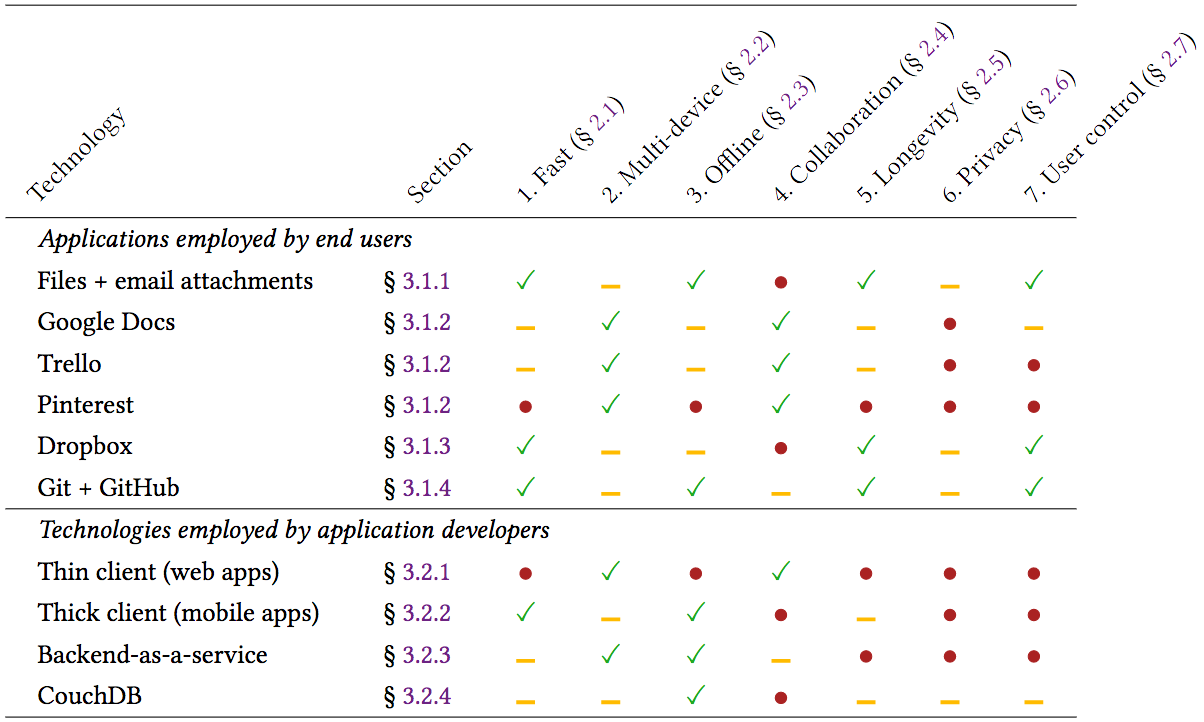
\includegraphics{img/lfs-comparison-apps}
  }
  \caption[Caption for lfs-comparison-apps]{Évaluation d'applications et de technologies vis-à-vis des 7 propriétés visées par les \acl{LFS}\footnotemark}
  \label{fig:lfs-comparison-apps}
\end{figure}

Malgré ce que ce résultat pourrait suggérer, les auteurs affirment que les fonctionnalités de collaboration entre utilisateur-rices ou même de synchronisation entre appareils ne sont pas antinomiques avec les propriétés de confidentialité, souveraineté, pérennité.

Ainsi, ils proposent un nouveau paradigme de conception d'applications collaboratives \ac{P2P}, nommées \acp{LFS}.
Ce paradigme vise à la conception d'applications offrant le meilleur des approches existantes, \ie cochant l'intégralité des critères de la \autoref{fig:lfs-comparison-apps}.
Nous partageons cette vision.\\
% Ce type d'applications se démarque de ceux existants, \eg les applications basées sur le cloud, par la place centrale donnée aux utilisateur-rices et leurs propres appareils, les éventuels serveurs étant relegués qu'à de simples rôles de support.

Cependant, de nombreuses problématiques de recherche identifiées dans \cite{localfirstsoftware2019} sont encore non résolues et entravent la démocratisation des applications \acp{LFS}.
Notamment, les applications \acp{LFS} se doivent de répliquer les données entre appareils pour permettre :
\begin{enumerate}
  \item Le fonctionnement en mode hors-ligne et le fonctionnement avec une faible latence.
  \item Le partage de contenu entre appareils d'un-e même utilisateur-rice.
  \item Le partage de contenu entre utilisateur-rices pour la collaboration.
\end{enumerate}

Toutefois, compte tenu des propriétés visées par les applications \acp{LFS}, plusieurs contraintes restreignent le choix des méthodes de réplication possibles.
Ainsi, pour permettre le fonctionnement en mode hors-ligne de l'application, \ie la consultation et la modification de contenu, les applications \acp{LFS} doivent relaxer la propriété de cohérence des données.
\begin{definition}[Cohérence]
  La cohérence d'un système indique sa capacité à présenter une vue uniforme de son état à chacun de ses utilisateur-rices à un moment donné.
\end{definition}

Les applications \acp{LFS} doivent donc adopter des méthodes de réplication dites optimistes \cite{2005-optimistic-replication-saito}.
Ces méthodes autorisent chaque noeud possédant une copie de la donnée de la consulter et de la modifier sans coordination au préalable avec les autres noeuds\footnote{Par opposition aux méthodes de réplication dites pessimistes, qui nécessitent une coordination préalable entre les noeuds avant toute modification de la donnée.}.
L'état des copies des noeuds peut donc diverger temporairement.
Un mécanisme de synchronisation permet ensuite aux noeuds de partager les modifications effectuées et de les intégrer de façon à converger à terme \cite{10.1145/224057.224070}, \ie obtenir à terme de nouveau des états équivalents.

Cependant, il convient de noter que les méthodes de réplication optimistes autorisent la génération en concurrence de modifications provoquant un conflit, \eg la modification et la suppression d'une même page dans un wiki.
Un mécanisme de résolution de conflits est alors nécessaire pour assurer la convergence à terme des noeuds.

De nouveau, le modèle du système des applications \acp{LFS} limitent les choix possibles concernant les mécanismes de résolution de conflits.
Notamment, les applications \acp{LFS} ne disposent d'aucun contrôle sur le nombre de noeuds qui compose le système, \ie le nombre d'appareils utilisés par l'ensemble de leurs utilisateur-rices.
\mnnote{TODO: Rattacher à la notion d'échelle des réseaux sociaux.}
Le nombre de noeuds peut donc croître de manière non-bornée.
La complexité algorithmique des mécanismes de résolution de conflits doit donc être indépendante de ce paramètre, ou alors en être fonction uniquement de manière logarithmique.

De plus, ces noeuds n'offrent aucune garantie sur leur stabilité.
Des noeuds peuvent donc rejoindre et participer au système, mais uniquement de manière éphèmère.
Ce phénonème est connu sous le nom de \emph{churn} \cite{understandingChurnP2PNetworks2006}.
Ainsi, de part l'absence de garantie sur le nombre de noeuds connectés de manière stable, les applications \acp{LFS} ne peuvent pas utiliser des mécanismes de résolution de conflits reposant sur une coordination synchrone d'une proportion des noeuds du système, \ie sur des algorithmes de consensus \cite{1998-paxos-lamport, 2014-raft-ongaro}.

Ainsi, pour permettre la conception d'applications \acp{LFS}, il convient de disposer de mécanismes de résolution de conflits pour l'ensemble des types de données avec une complexité algorithmique efficace par rapport au nombre de noeuds et ne nécessitant pas de coordination synchrone entre une proportion des noeuds du système.

% \subsection{Réplication de données mutables}

% Les techniques de réplication de données mutables introduisent de la redondance de données dans les systèmes.
% Cette redondance a pour but et effet d'améliorer plusieurs propriétés des systèmes :

% \begin{definition}[Disponibilité]
% \end{definition}

% \begin{definition}[Tolérance aux pannes]
% \end{definition}

% \begin{definition}[Capacité de passage à l'échelle]
% \end{definition}

% \begin{definition}[Latence]
% \end{definition}

% Les techniques de réplication de données peuvent être classées en deux approches : les \emph{techniques de réplication de données pessimistes} et les \emph{techniques de réplication de données optimistes}.
% Ces deux catégories offrent des compromis différents vis-à-vis des propriétés décrites par les théorèmes CAP \cite{brewer_2000_podc} et PACELC \cite{pacelc2012}.
% Notamment, la différence entre ces catégories concerne le cas de la propriété de \emph{cohérence}.

% \begin{definition}[Cohérence]
% \end{definition}

% \subsection{Réplication de données pessimiste}

% Les techniques de réplication de données dites \emph{pessimistes} privilègie la cohérence des données.
% Notamment, ces techniques empêchent les modifications en concurrence d'une même donnée.
% Pour cela, plusieurs approches sont possibles.

% \begin{itemize}
%     \item Première approche consiste à utiliser un verrou.
%     \item Seconde approche consiste à utiliser un système de vote pour décider de la prochaine modification.
%         Consensus, élection de leader, SMR.
%     \item Le choix de privilégier la cohérence des données se fait au détriment de la disponibilité, tolérance aux pannes, capacité de passage à l'échelle et latence.
%         Par exemple, un système basé sur un leader deviendra temporairement indisponible lors d'une panne de son leader, le temps que la panne soit détectée et qu'un nouveau leader soit élu.
% \end{itemize}

% \subsection{Réplication de données optimiste}

% À l'inverse, les techniques de réplication de données dites \emph{optimistes} jugent acceptable de relâcher les contraintes existantes sur la cohérence des données.
% Dans ce paradigme, chaque noeud qui possède une copie de la donnée répliquée peut la consulter et la modifier à tout moment, sans coordination préalable avec les autres noeuds.
% Les copies des noeuds sont donc autorisées à diverger de manière temporaire.

% Les modifications effectuées par chacun sont ensuite diffusées pour être intégrées par l'ensemble des noeuds et converger de nouveau, \ie atteindre des états équivalents.
% Cependant, certaines modifications effectuées en concurrence par les noeuds peuvent provoquer des conflits.
% \mnnote{NOTE: Pourrait insérer exemple de conflits de l'édition collaborative ici.}
% Des mécanismes de résolution de conflits, potentiellement automatiques, sont alors requis pour assurer la convergence à terme.

% Cette approche permet donc de privilégier la disponibilité, tolérance aux pannes, capacité de passage à l'échelle et latence en échange de la cohérence forte.

% Dans le cadre de cette thèse, nous nous intéressons aux techniques de réplication de données optimistes.


\section{Questions de recherche et contributions}
\subsection{Ré-identification sans coordination synchrone pour les \acp{CRDT} pour le type Séquence}
\label{sec:research-questions-rls}

Les \acfp{CRDT}\footnote{\acf{CRDT} : Type de données répliquées sans conflits} \cite{2007-crdt-shapiro,shapiro_2011_crdt} sont des nouvelles spécifications des types de données usuels, \eg l'Ensemble ou la Séquence.
Ils sont conçus pour permettre à un ensemble de noeuds d'un système de répliquer une donnée et pour leur permettre de la consulter, de la modifier sans aucune coordination préalable et d'assurer à terme la convergence des copies.
Dans ce but, les \acp{CRDT} incorporent des mécanismes de résolution de conflits automatiques directement au sein leur spécification.

Cependant, ces mécanimes induisent un surcoût, aussi bien en termes de métadonnées et de calculs que de bande-passante.
Ces surcoûts sont néanmoins jugés acceptables par la communauté pour une variété de types de données, \eg le Registre ou l'Ensemble.
Cependant, le surcoût des \acp{CRDT} pour le type Séquence constitue toujours une problématique de recherche.

En effet, la particularité des \acp{CRDT} pour le type Séquence est que leur surcoût croît de manière monotone au cours de la durée de vie de la donnée, \ie au fur et à mesure des modifications effectuées.
Le surcoût introduit par les \acp{CRDT} pour ce type de données se révèle donc handicapant dans le contexte de collaborations sur de longues durées ou à large échelle.

De manière plus précise, le surcoût des \acp{CRDT} pour le type Séquence provient de la croissance des métadonnées utilisées par leur mécanisme de résolution de conflits automatique.
Ces métadonnées correspondent à des identifiants qui sont associés aux éléments de la Séquence.
Ces identifiants permettent d'intégrer les modifications, \eg en précisant quel est l'élément à supprimer ou en spécifiant la position d'un nouvel élément à insérer par rapport aux autres.

Plusieurs approches ont été proposées pour réduire le coût induit par ces identifiants.
Notamment, \cite{letia:hal-01248270,zawirski:hal-01248197} proposent un mécanisme de ré-assignation des identifiants pour réduire leur coût a posteriori.
Ce mécanisme génère toutefois des conflits en cas de modifications concurrentes de la séquence, \ie l'insertion ou la suppression d'un élément.
Les auteurs résolvent ce problème en proposant un mécanisme de transformation des modifications concurrentes par rapport à l'effet du mécanisme de ré-assignation des identifiants.

Cependant, l'exécution en concurrence du mécanisme de ré-assignation des identifiants par plusieurs noeuds provoque elle-même un conflit.
Pour éviter ce dernier type de conflit, les auteurs choisissent de subordonner à un algorithme de consensus l'exécution du mécanisme de ré-assignation des identifiants.
Ainsi, le mécanisme de ré-assignation des identifiants ne peut être déclenché en concurrence par plusieurs noeuds du système.

Comme nous l'avons évoqué précédemment, reposer sur un algorithme de consensus qui requiert une coordination synchrone entre une proportion de noeuds du système est une contrainte incompatible avec les systèmes \ac{P2P} à large échelle sujets au churn.\\

Notre problématique de recherche est donc la suivante : \emph{pouvons-nous proposer un mécanisme sans coordination synchrone de réduction du surcoût des \acp{CRDT} pour le type Séquence, \ie adapté aux applications \ac{LFS} ?}\\

Pour répondre à cette problématique, nous proposons dans cette thèse RenamableLogootSplit, un nouveau \ac{CRDT} pour le type Séquence.
Ce \ac{CRDT} intègre un mécanisme de ré-assignation des identifiants, dit de renommage, directement au sein de sa spécification.
Nous associons au mécanisme de renommage un mécanisme de résolution de conflits automatique additionnel pour gérer ses exécutions concurrentes.
Finalement, nous définissons un mécanisme de \acf{GC}\footnote{\acf{GC} : Récupération de la mémoire} des métadonnées du mécanisme de renommage pour supprimer à terme son propre surcoût.
De cette manière, nous proposons un \ac{CRDT} pour le type Séquence dont le surcoût est périodiquement réduit, tout en n'introduisant aucune contrainte de coordination synchrone entre les noeuds du système.

\subsection{Éditeur de texte collaboratif \ac{P2P} temps réel chiffré de bout en bout}
\label{sec:research-questions-mute}

Comme évoqué précédemment, la conception d'applications \ac{LFS} à large échelle présente un ensemble de problématiques issues de domaines variés, \eg
\begin{enumerate}
    \item Comment permettre aux utilisateur-rices de collaborer en l'absence d'autorités centrales pour résoudre les conflits de modifications ?
    \item Comment authentifier les utilisateur-rices en l'absence d'autorités centrales ?
    \item Comment structurer le réseau de manière efficace, \ie en limitant le nombre de connexions par pair ?
\end{enumerate}

Cet ensemble de questions peut être résumé en la problématique suivante : \emph{pouvons-nous concevoir une application \ac{LFS} à large échelle, sûre et sans autorités centrales ?}\\

Pour étudier cette problématique, l'équipe Coast développe l'application \acf{MUTE}\footnote{Disponible à l'adresse : \url{https://mutehost.loria.fr}} \cite{MUTE2017}.
Il s'agit d'un \acf{PoC}\footnote{\acf{PoC} : Preuve de concept} d'éditeur de texte web collaboratif \ac{P2P} temps réel chiffré de bout en bout.
Ce projet permet à l'équipe de présenter ses travaux de recherche portant sur les mécanismes de résolutions de conflits automatiques pour le type Séquence \cite{2013-logootsplit,2021-these-vic,2022-rls-tpds-nicolas} et les mécanismes d'authentification des pairs dans les systèmes sans autorités centrales \cite{2018-trusternity-short,2018-trusternity-long}.

De plus, en inscrivant ses travaux dans le cadre d'un système complet, ce projet permet à l'équipe d'identifier de nouvelles problématiques en relation avec les nombreux domaines de recherche nécessaires à la conception d'un tel système, \eg le domaine des protocoles d'appartenance aux groupes \cite{swim2002, lifeguard2018}, des topologies réseaux \ac{P2P} \cite{2018-spray-nedelec} ou encore des protocoles d'établissement de clés de chiffrement de groupe \cite{1995-burmester-desmedt}.\\

Dans le cadre de cette thèse, nous avons contribué au développement de ce projet.
Nous avons notamment implémenté plusieurs \acp{CRDT} pour le type Séquence \cite{2013-logootsplit,2022-rls-tpds-nicolas} et le protocole d'appartenance au réseau SWIM \cite{swim2002}.


\section{Plan du manuscrit}
\begin{itemize}
    \item Ce manuscrit de thèse est organisé de la manière suivante :
    \item Dans le \autoref{chap:state-of-art}, nous introduisons le modèle du système que nous considérons, \ie les systèmes \ac{P2P} à large échelle sujet au churn.
        Puis nous présentons dans ce chapitre l'état de l'art des mécanismes de résolution de conflits automatiques utilisés dans les systèmes adoptant le paradigme de la réplication optimiste.
        À partir de cet état de l'art, nous identifions et motivons notre problématique de recherche, \ie l'absence de mécanisme adapté aux systèmes \ac{P2P} à large échelle sujet au churn permettant de réduire le surcoût induit par les mécanismes de résolution de conflits automatiques pour le type Séquence.
    \item Dans le \autoref{chap:renamablelogootsplit}, nous présentons notre approche pour présenter un tel mécanisme, \ie un mécanisme de résolution de conflits automatiques pour le type Séquence auquel nous associons un mécanisme de \ac{GC} de son surcoût ne nécessitant pas de coordination synchrone entre les noeuds du système.
        Nous détaillons le fonctionnement de notre approche, sa validation par le biais d'une évaluation empirique puis comparons notre approche par rapport aux approches existantes
        Finalement, nous concluons la présentation de notre approche en identifiant et en détaillant plusieurs de ses limites.
    \item Dans le \autoref{chap:mute}, nous présentons \ac{MUTE}, l'éditeur de texte collaboratif temps réel \ac{P2P} chiffré de bout en bout que notre équipe de recherche développe dans le cadre de ses travaux de recherche.
        Nous présentons les différentes couches logicielles formant un pair et les services tiers avec lesquels les pairs interagissent, et détaillons nos travaux dans le cadre de ce projet, \ie l'intégration de notre mécanisme de résolution de conflits automatiques pour le type Séquence et le développement de la couche de livraison des messages associée.
        Pour chaque couche logicielle, nous identifions ses limites et présentons de potentielles pistes d'améliorations.
    \item Finalement, nous récapitulons dans le \autoref{chap:conclusions-perspectives} les contributions réalisées dans le cadre de cette thèse.
        Puis nous clotûrons ce manuscrit en introduisant plusieurs des pistes de recherches que nous souhaiterons explorer dans le cadre de nos travaux futurs.
\end{itemize}


\section{Publications}
Notre travail sur la problématique identifiée dans la \autoref{sec:research-questions-rls}, \ie la proposition d'un mécanisme ne nécessitant aucune coordination synchrone pour réduire le surcoût des \acp{CRDT} pour le type Séquence, a donné lieu à des publications à différents stades de son avancement :
\begin{enumerate}
    \item Dans \cite{2018-rls-middleware-nicolas}, nous motivons le problème identifié et présentons l'idée de notre approche pour y répondre.
    \item Dans \cite{2020-rls-papoc-nicolas}, nous détaillons une première partie de notre approche et présentons notre protocole d'évaluation expérimentale ainsi que ses premiers résultats.
    \item Dans \cite{2022-rls-tpds-nicolas}, nous détaillons notre proposition dans son entièreté.
        Nous accompagnons cette proposition d'une évaluation expérimentale poussée.
        Finalement, nous complétons notre travail d'une discussion analysant ses limites connues et présentant des pistes de travail possibles pour y répondre.
\end{enumerate}
Nous précisons ci-dessous les informations relatives à chacun de ces articles.

\subsection*{Efficient renaming in CRDTs \cite{2018-rls-middleware-nicolas}}

\paragraph{Auteur} Matthieu Nicolas

\paragraph{Article de position} à Middleware 2018 - 19th ACM/IFIP International Middleware Conference (Doctoral Symposium), Dec 2018, Rennes, France.

\paragraph{Abstract}
\emph{Sequence Conflict-free Replicated Data Types (CRDTs)} allow to replicate and edit, without any kind of coordination, sequences in distributed systems.
To ensure convergence, existing works from the literature add metadata to each element but they do not bound its footprint, which impedes their adoption.
Several approaches were proposed to address this issue but they do not fit a fully distributed setting.
In this paper, we present our ongoing work on the design and validation of a fully distributed renaming mechanism, setting a bound to the metadata's footprint.
Addressing this issue opens new perspectives of adoption of these CRDTs in distributed applications.

\subsection*{Efficient Renaming in Sequence CRDTs \cite{2020-rls-papoc-nicolas}}

\paragraph{Auteurs} Matthieu Nicolas, Gérald Oster, Olivier Perrin

\paragraph{Article de workshop} à PaPoC 2020 - 7th Workshop on Principles and Practice of Consistency for Distributed Data, Apr 2020, Heraklion / Virtual, Greece.

\paragraph{Abstract}
To achieve high availability, large-scale distributed systems have to replicate data and to minimise coordination between nodes.
Literature and industry increasingly adopt \acfp{CRDT} to design such systems.
\acp{CRDT} are data types which behave as traditional ones, e.g. the Set or the Sequence.
However, unlike traditional data types, they are designed to natively support concurrent modifications.
To this end, they embed in their specification a conflict-resolution mechanism.

To resolve conflicts in a deterministic manner, \acp{CRDT} usually attach identifiers to elements stored in the data structure.
Identifiers have to comply with several constraints, such as uniqueness or belonging to a dense order.
These constraints may hinder the identifiers’ size from being bounded.
As the system progresses, identifiers tend to grow.
This inflation deepens the overhead of the \ac{CRDT} over time, leading to performance issues.

To address this issue, we propose a new CRDT for Sequence which embeds a renaming mechanism.
It enables nodes to reassign shorter identifiers to elements in an uncoordinated manner.
Experimental results demonstrate that this mechanism decreases the overhead of the replicated data structure and eventually limits it.

\subsection*{Efficient Renaming in Sequence CRDTs \cite{2022-rls-tpds-nicolas}}

\paragraph{Auteurs} Matthieu Nicolas, Gérald Oster, Olivier Perrin

\paragraph{Article de journal} dans IEEE Transactions on Parallel and Distributed Systems, Institute of Electrical and Electronics Engineers, 2022, 33 (12), pp.3870-3885.

\paragraph{Abstract}
To achieve high availability, large-scale distributed systems have to replicate data and to minimise coordination between nodes.
For these purposes, literature and industry increasingly adopt \acfp{CRDT} to design such systems.
\acp{CRDT} are new specifications of existing data types, e.g. Set or Sequence.
While \acp{CRDT} have the same behaviour as previous specifications in sequential executions, they actually shine in distributed settings as they natively support concurrent updates.
To this end, \acp{CRDT} embed in their specification conflict resolution mechanisms.
These mechanisms usually rely on identifiers attached to elements of the data structure to resolve conflicts in a deterministic and coordination-free manner.
Identifiers have to comply with several constraints, such as being unique or belonging to a dense total order.
These constraints may hinder the identifier size from being bounded.
Identifiers hence tend to grow as the system progresses, which increases the overhead of \acp{CRDT} over time and leads to performance issues.
To address this issue, we propose a novel Sequence \ac{CRDT} which embeds a renaming mechanism.
It enables nodes to reassign shorter identifiers to elements in an uncoordinated manner.
Experimental results demonstrate that this mechanism decreases the overhead of the replicated data structure and eventually minimises it.


\import{chapters/etat-art/}{etat-art}
% \import{chapters/rls/}{rls}
% \import{chapters/mute/}{mute}

\NumberThisInToc
\chapter{Conclusions et perspectives}
\minitoc
\label{chap:conclusions-perspectives}


Dans ce chapitre, nous revenons sur les contributions présentées dans cette thèse.
Nous rappelons le contexte dans lequel elles s'inscrivent, récapitulons leurs spécificités et apports, et finalement précisons plusieurs de leurs limites.
Puis, nous concluons ce manuscrit en présentant plusieurs pistes de recherche qui nous restent à explorer à l'issue de cette thèse.
La première s'inscrit dans la continuité directe de nos travaux sur un mécanisme de ré-identification pour \acp{CRDT} pour le type Séquence pour les applications \acf{LFS}.
Les dernières traduisent quant à elles notre volonté de recentrer nos travaux sur le domaine plus général des \acp{CRDT}.


\section{Résumés des contributions}

\subsection{Réflexions sur l'état de l'art des \acp{CRDT}}
Les \acfp{CRDT} \cite{shapiro_2011_crdt} sont de nouvelles spécifications des types de données.
Ils sont conçus pour permettre à un ensemble de noeuds d'un système de répliquer une même donnée et pour leur permettre de la consulter et de la modifier sans aucune coordination préalable.
Les copies des noeuds divergent alors temporairement.
Les noeuds se synchronisent ensuite pour s'échanger leurs modifications respectives.
Les \acp{CRDT} garantissent alors la cohérence forte à terme \cite{shapiro_2011_crdt}, \ie que les noeuds obtiennent de nouveau des copies équivalentes de la donnée.

L'absence de coordination entre les noeuds avant modifications implique que des noeuds peuvent modifier la donnée en concurrence.
De telles modifications peuvent donner lieu à des conflits, \eg l'ajout et la suppression en concurrence d'un même élément dans un ensemble.
Pour pallier ce problème, les \acp{CRDT} incorporent un mécanisme de résolution de conflits automatiques directement au sein de leur spécification.

Il convient de noter qu'il existe plusieurs solutions possibles pour résoudre un conflit.
Pour reprendre l'exemple de l'élément ajouté et supprimé en concurrence d'un ensemble, nous pouvons par exemple soit le conserver l'élément, soit le supprimer.
Nous parlons alors de sémantique du mécanisme de résolution de conflits automatique.

De la même manière, il existe plusieurs approches possibles pour synchroniser les noeuds, \eg diffuser chaque modification de manière atomique ou diffuser l'entièreté de l'état périodiquement.
Ainsi, lors de la définition d'un \ac{CRDT}, il convient de préciser les sémantiques de résolution de conflits qu'il adopte et le modèle de synchronisation qu'il utilise \cite{2018-crdts-overview-preguica}.\\

Depuis leur formalisation, de nombreux travaux ont abouti à la conception de nouveaux \acp{CRDT}, soit en spécifiant de nouvelles sémantiques de résolution de conflits pour un type de données \cite{2020-cl-set-weihai}, soit en spécifiant de nouveaux modèles de synchronisation \cite{Almeida_2018} ou en enrichissant les spécifications des modèles existants \cite{baquero2017pure,enes2019}.

Dans notre présentation des \acp{CRDT} \cf{sec:etat-art-crdts-intro}, nous présentons chacun de ces aspects.
Cependant, nous nous ne limitons pas à retranscrire l'état de l'art de la littérature.
Notamment au sujet du modèle de synchronisation par opérations, nous précisons que le modèle de livraison causal n'est pas nécessaire pour l'ensemble des \acp{CRDT} synchronisés par opérations, \ie que certains peuvent adopter des modèles de livraison moins contraints et donc moins coûteux.
Cette précision nous permet de proposer une étude comparative des différents modèles de synchronisation qui est, à notre connaissance, l'une des plus précises de la littérature \cf{def:synchro-synthese}.\\

Nous présentons ensuite les différents \acp{CRDT} pour le type Séquence de la littérature \cf{sec:seq-crdts}.
Nous mettons alors en exergue les deux approches proposées pour concevoir le mécanisme de résolution de conflits automatiques pour le type Séquence, \ie l'approche à pierres tombales et l'approche à identifiants densément ordonnés.
De nouveau, cette rétrospective nous permet d'expliciter des angles morts des articles d'origine, notamment vis-à-vis des modèle de livraison des opérations des \acp{CRDT} proposés.
Puis, nous mettons en lumière les limites des évaluations comparant les deux approches, \ie le couplage entretenu entre approche du mécanisme de résolution de conflits et choix d'implémentations.
Cette limite empêche d'établir la supériorité d'une des approches par rapport à l'autre.
Finalement, nous conjecturons que le surcoût de ces deux approches est le même, \ie le coût nécessaire à la représentation d'un espace dense.
Nous précisons dès lors par le biais de notre propre étude comparative comment ce surcoût s'exprime dans chacune des approches , \ie le compromis entre surcoût en métadonnées, calculs et bande-passante proposé par les deux approches \cf{sec:seq-crdts-synth}.\\

Ces réflexions que nous présentons sur l'état des \acp{CRDT} définissent plusieurs pistes de recherches.
Une première d'entre elles concerne notre étude comparative des modèles de synchronisation.
D'après les critères que nous utilisons, une conclusion possible de cette comparaison est que le modèle de synchronisation par différences d'états rend obsolètes les modèles de synchronisation par états et par opérations.
En effet, le modèle de synchronisation par différences d'états apparaît comme adapté à l'ensemble des contextes d'utilisation qui étaient jusqu'alors exclusifs à ces derniers, de par les multiples stratégies qu'il permet, \eg synchronisation par états complets, synchronisation par états irréductibles...

Cette conclusion nous paraît cependant hâtive.
Il convient d'étendre notre étude comparative pour prendre en compte des critères de comparaison additionnels pour confirmer cette conjecture, ou l'invalider et définir plus précisément les spécificités de chacun des modèles de synchronisation.
Nous détaillons cette piste de recherche dans la \autoref{sec:perspective-comparison-sync-models}.\\

Une seconde piste de recherche possible concerne les deux approches utilisées pour concevoir le mécanisme de résolution de conflits des \acp{CRDT} pour le type Séquence.
Comme dit précédemment, nous conjecturons que ces deux approches ne sont finalement que deux manières différentes de représenter une même information : la position d'un élément dans un espace dense.
La différence entre ces approches résiderait uniquement dans la manière que chaque représentation influe sur les performances du \ac{CRDT}.
Une piste de travail serait donc de confirmer cette conjecture, en proposant une formalisation unique des \acp{CRDT} pour le type Séquence.


\subsection{Ré-identification sans coordination pour les \acp{CRDT} pour Séquence}
Pour privilégier leur disponibilité, latence et tolérance aux pannes, les systèmes distribués peuvent adopter le paradigme de la réplication optimiste \cite{2005-optimistic-replication-saito}.
Ce paradigme consiste à relaxer la cohérence de données entre les noeuds du système pour leur permettre de consulter et modifier leur copie locale sans se coordonner.
Leur copies peuvent alors temporairement diverger avant de converger de nouveau une fois les modifications de chacun propagées.
Cependant, cette approche nécessite l'emploi d'un mécanisme de résolution de conflits pour assurer la convergence même en cas de modifications concurrentes.
Pour cela, l'approche des \acp{CRDT} \cite{2007-crdt-shapiro,shapiro_2011_crdt} propose d'utiliser des types de données dont les modifications sont nativement commutatives.

Depuis la spécification des \acp{CRDT}, la littérature a proposé plusieurs de ces mécanismes résolution de conflits automatiques pour le type de données Séquence \cite{2006-woot-oster,ROH2011354,2009-treedoc-preguica,2009-logoot-weiss}.
Cependant, ces approches souffrent toutes d'un surcoût croissant de manière monotone.
Ce problème a été identifié par la communauté, et celle-ci a proposé pour y répondre des mécanismes permettant soit de réduire la croissance du surcoût \cite{lseq2013,lseq2017}, soit d'effectuer une \ac{GC} du surcoût \cite{ROH2011354,letia:hal-01248270,zawirski:hal-01248197}.
Nous avons cependant déterminé que ces mécanismes ne sont pas adaptés aux systèmes \ac{P2P} à large échelle souffrant de churn et utilisant des \acp{CRDT} pour Séquence à granularité variable.

Dans le cadre de cette thèse, nous avons donc souhaité proposer un nouveau mécanisme adapté à ce type de systèmes.
Pour cela, nous avons suivi l'approche proposée par \cite{letia:hal-01248270,zawirski:hal-01248197} : l'utilisation d'un mécanisme pour ré-assigner de nouveaux identifiants aux élements stockées dans la séquence.
Nous avons donc proposé un nouveau mécanisme appartenant à cette approche pour le \ac{CRDT} LogootSplit \cite{2013-logootsplit}.\\

Notre proposition prend la forme d'un nouvel \ac{CRDT} pour Séquence à granularité variable : RenamableLogootSplit.
Ce nouveau \ac{CRDT} associe à LogootSplit un nouveau type de modification, $\trm{ren}$, permettant de produire une nouvelle séquence équivalente à son état précédent.
Cette nouvelle modification tire profit de la granularité variable de la séquence pour produire un état de taille minimale : elle assigne à tous les éléments des identifiants de position issus d'un même intervalle.
Ceci nous permet de minimiser les métadonnées que la séquence doit stocker de manière effective.
% De plus, le passage à une représentation interne minimale de la séquence nous permet d'améliorer le coût des modifications suivantes en termes de calculs.

Afin de gérer les opérations concurrentes aux opérations $\trm{ren}$, nous définissons pour ces dernières un algorithme de transformation.
Pour cela, nous définissons un mécanisme d'époques nous permettant d'identifier la concurrence entre opérations.
De plus, nous introduisons une relation d'ordre strict total, \emph{priority}, pour résoudre de manière déterministe le conflit provoqué par deux opérations $\trm{ren}$, \ie pour déterminer quelle opération $\trm{ren}$ privilégier.
Finalement, nous définissons deux algorithmes, \texttt{renameId} et \texttt{revertRenameId}, qui permettent de transformer les opérations concurrentes à une opération $\trm{ren}$ pour prendre en compte l'effet de cette dernière.
Ainsi, notre algorithme permet de détecter et de transformer les opérations concurrentes aux opérations $\trm{ren}$, sans nécessiter une coordination synchrone entre les noeuds.\\


Pour valider notre approche, nous proposons une évaluation expérimentale de cette dernière.
Cette évaluation se base sur des traces de sessions d'édition collaborative que nous avons généré par simulations.
Chacune de ces simulations représente la rédaction collaborative d'un document texte par 10 noeuds.

Notre évaluation nous permet de valider de manière empirique les résultats attendus.
Le premier d'entre eux concerne la convergence des noeuds.
En effet, nos simulations nous ont permis de valider que l'ensemble des noeuds obtenaient des états finaux équivalents, même en cas d'opérations $\trm{ren}$ concurrentes.

Notre évaluation nous a aussi permis de valider que le mécanisme de renommage réduit à une taille minimale le surcoût du mécanisme de résolution de conflits incorporé dans le \ac{CRDT} pour Séquence.

L'évaluation expérimentale nous a aussi permis de prendre conscience d'effets additionnels du mécanisme de renommage que nous n'avions pas anticipé.
Notamment, elle montre que le surcoût éventuel du mécanisme de renommage, notamment en termes de calculs, est toutefois contrebalancé par l'amélioration précisée précédemment, \ie la réduction de la taille de la séquence.\\

Finalement, notons que le mécanisme que nous proposons est partiellement générique : il peut être adapté à d'autres \acp{CRDT} pour Séquence à granularité variable, \eg un \ac{CRDT} pour Séquence appartenant à l'approche à pierres tombales.
Dans le cadre d'une telle démarche, nous pourrions réutiliser le système d'époques, la relation \emph{priority} et l'algorithme de contrôle qui identifie les transformations à effectuer.
Pour compléter une telle adaptation, nous devrions cependant concevoir de nouveaux algorithmes \texttt{renameId} et \texttt{revertRenameId} spécifiques et adaptés au \ac{CRDT} choisi.\\

Le mécanisme de renommage que nous présentons souffre néanmoins de plusieurs limites.
La première d'entre elles concerne ses performances.
En effet, notre évaluation expérimentale a mis en lumière le coût important en l'état de la modification $\trm{ren}$ par rapport aux autres modifications en termes de calculs \cf{sec:integration-time-rename}.
De plus, chaque opération $\trm{ren}$ comporte une représentation de l'ancien état qui doit être maintenue par les noeuds jusqu'à leur stabilité causale.
Le surcoût en métadonnées introduit par un ensemble d'opérations $\trm{ren}$ concurrentes peut donc s'avérer important, voire pénalisant \cf{sec:evaluation-metadata}.
Pour répondre à ces problèmes, nous identifions trois axes d'amélioration :
\begin{enumerate}
    \item La définition de stratégies de déclenchement du renommage efficaces.
        Le but de ces stratégies serait de déclencher le mécanisme de renommage de manière fréquente, de façon à garder son temps d'exécution acceptable, mais tout visant à minimiser la probabilité que les noeuds produisent des opérations $\trm{ren}$ concurrentes, de façon à minimiser le surcoût en métadonnées.
    \item La définition de relations \emph{priority} efficaces.
        Nous développons ce point dans la \autoref{sec:alternative-priority}.
    \item La proposition d'algorithmes de renommage efficaces.
        Cette amélioration peut prendre la forme de nouveaux algorithmes pour \texttt{renameId} et \texttt{revertRenameId} offrant une meilleure complexité en temps.
        Il peut aussi s'agir de la conception d'une nouvelle approche pour renommer l'état et gérer les modifications concurrentes, \eg un mécanisme de renommage basé sur le journal des opérations \cf{sec:log-based-rename-mechanism}.
\end{enumerate}

Une seconde limite de RenamableLogootSplit que nous identifions concerne son mécanisme de \ac{GC} des métadonnées introduites par le mécanisme de renommage.
En effet, pour fonctionner, ce dernier repose sur la stabilité causale des opérations $\trm{ren}$.
Pour rappel, la stabilité causale représente le contexte causal commun à l'ensemble des noeuds du système.
Pour le déterminer, chaque noeud doit récupérer le contexte causal de l'ensemble des noeuds du système.
Ainsi, l'utilisation de la stabilité causale comme pré-requis pour la \ac{GC} de métadonnées constitue une contrainte forte, voire prohibitive, dans les systèmes \ac{P2P} à large échelle sujet au churn.
En effet, un noeud du système déconnecté de manière définitive suffit pour empêcher la stabilité causale de progresser, son contexte causal étant alors indéterminé du point de vue des autres noeuds.
Il s'agit toutefois d'une limite récurrente des mécanismes de \ac{GC} distribués et asynchrones \cite{ROH2011354,baquero2017pure,2018-prunable-authenticated-log-vic}.
Nous présentons une piste de travail possible pour pallier ce problème dans la \autoref{sec:manual-merge}.


\subsection{Éditeur de texte collaboratif \ac{P2P} chiffré de bout en bout}
Les applications collaboratives permettent à des utilisateur-rices de réaliser collaborativement une tâche.
Elles permettent à plusieurs utilisateur-rices de consulter la version actuelle du document, de la modifier et de partager leurs modifications avec les autres.
Ceci permet de mettre en place une réflexion de groupe, ce qui améliore la qualité du résultat produit \cite{2004-empirical-study-collaborative-writing,2005-internet-encyclopaedias-head-to-head}.

Cependant, les applications collaboratives sont historiquement des applications centralisées, \eg Google Docs \cite{gdocs}.
Ce type d'architecture induit des défauts d'un point de vue technique, \eg faible capacité de passage à l'échelle et faible tolérance aux pannes, mais aussi d'un point de vue utilisateur, \eg perte de la souveraineté des données et absence de garantie de pérennité.\\

Les travaux de l'équipe Coast s'inscrivent dans une mouvance souhaitant résoudre ces problèmes et qui a conduit à la définition d'un nouveau paradigme d'applications : les applications \acf{LFS} \cite{localfirstsoftware2019}.
Le but de ce paradigme est la conception d'applications collaboratives, \ac{P2P}, pérennes et rendant la souveraineté de leurs données aux utilisateur-rices.

Dans le cadre de cette démarche, l'équipe Coast développe depuis plusieurs années l'application \acf{MUTE}, un éditeur de texte web collaboratif \ac{P2P} temps réel chiffré de bout en bout.
Cette application sert à la fois de plateforme de démonstration et de recherche pour les travaux de l'équipe, mais aussi de \acf{PoC} pour les \ac{LFS}.
Ainsi, \ac{MUTE} propose au moment où nous écrivons ces lignes un aperçu des travaux de recherche existants concernant :
\begin{enumerate}
    \item Les mécanismes de résolution de résolutions de conflits automatiques pour l'édition collaborative de documents textes \cite{2013-logootsplit,2021-these-vic,2022-rls-tpds-nicolas}.
    \item Les protocoles distribués d'appartenance au groupe \cite{swim2002}.
    \item Les mécanismes d'anti-entropie \cite{1983-anti-entropy-vv}.
    \item Les protocoles distribués d'authentification d'utilisateur-rices \cite{2018-trusternity-short,2018-trusternity-long}.
    \item Les protocoles distribués d'établissement de clés de chiffrement de groupe \cite{1995-burmester-desmedt}.
    \item Les mécanismes de conscience de groupe.
\end{enumerate}
Dans cette liste, nous avons personnellement contribué à l'implémentation des \acp{CRDT} LogootSplit \cite{2013-logootsplit} et RenamableLogootSplit \cite{2022-rls-tpds-nicolas}, et du protocole d'appartenance au groupe SWIM \cite{swim2002}.\\

En son état actuel, \ac{MUTE} présente cependant plusieurs limites.
Tout d'abord, l'environnement web implique un certain nombre de contraintes, notamment au niveau des technologies et protocoles disponibles.
Notamment, le protocole \acf{WebRTC} repose sur l'utilisation de serveurs de signalisation, \ie de points de rendez-vous des pairs, et de serveurs de relais, \ie d'intermédiaires pour communiquer entre pairs lorsque les configurations de leur réseaux respectifs interdisent l'établissement d'une connexion directe.
Ainsi, les applications \ac{P2P} web doivent soit déployer et maintenir leur propre infrastructure de serveurs, soit reposer sur une infrastructure existante, \eg celle proposée par OpenRelay \cite{openrelay}.

Dans le cadre de \ac{MUTE}, nous avons opté pour cette seconde solution.
Cependant, ce choix introduit un \acf{SPOF}\footnote{\acf{SPOF} : Point de défaillance unique} dans \ac{MUTE} : OpenRelay elle-même.
Afin de garantir la pérennité de \ac{MUTE}, nous devrions reposer non pas sur une unique infrastructure de serveurs de signalisation et de relais mais sur une multitude.
Malheureusement, l'écosystème actuel brille par la rareté d'infrastructures publiques offrant ces services.
Nous devons donc encourager et supporter la mise en place de telles infrastructures par une pluralité d'organisations.\\

Une autre limite de ce système que nous identifions concerne l'utilisabilité des systèmes \ac{P2P} de manière générale.
L'expérience vécue suivante constitue à notre avis un exemple éloquent des limites actuelles de l'application \ac{MUTE} dans ce domaine.
Après avoir rédigé une version initiale d'un document, nous avons envoyé le lien du document à notre collaborateur pour relecture et validation.
Lorsque notre collaborateur a souhaité accéder au document, celui-ci s'est retrouvé devant une page blanche : comme nous nous étions déconnecté du système entretemps, plus aucun pair possédant une copie n'était disponible pour se synchroniser.

Notre collaborateur était donc dans l'incapacité de récupérer le document et d'effectuer sa tâche.
Afin de pallier ce problème, une solution possible est de faire reposer \ac{MUTE} sur un réseau \ac{P2P} global, \eg le réseau de \ac{IPFS} \cite{ipfs}, et d'utiliser les pairs de ce dernier, potentiellement des pairs étrangers à l'application, comme pairs de stockage pour permettre une synchronisation future.
Cette solution limiterait ainsi le risque qu'un pair ne puisse récupérer l'état du document faute de pairs disponibles.
Pour garantir l'utilisabilité du système \ac{P2P}, une telle solution devrait donc permettre à un pair de récupérer l'état du document à sa reconnexion, malgré la potentielle évolution du groupe des collaborateur-rices et des pairs de stockage, \eg l'ajout, l'éviction ou la déconnexion d'un des pairs.
Cependant, la solution devrait en parallèle garantir qu'elle n'introduit aucune vulnérabilité, \eg la possibilité pour les pairs de stockage selectionnés de reconstruire et consulter le document.
% \item Finalement, une dernière limite que nous identifions est la pérennité économique de ce type d'applications.
%     Selon nous, les systèmes \ac{P2P} chiffrés de bout en bout s'interdisent les modèles économiques dominants et acceptés par les organisations et utilisateur-rices, \ie la collecte et revente de données.
%     En effet,
%     , de par les propriétés qu'ils assurent, notamment la confidentialité des données .
%     \mnnote{TODO: Voir si on a des données sur les entreprises/organisations encourageant le chiffrement de bout-en-bout dans leurs outils internes, }


\section{Perspectives}

\subsection{Définition de relations de priorité pour minimiser les traitements}
\label{sec:alternative-priority}

Dans la \autoref{sec:priority}, nous avons spécifié la relation \emph{priority} \cf{def:priority-relation}.
Pour rappel, cette relation doit établir un ordre strict total sur les époques de notre mécanisme de renommage.

Cette relation nous permet ainsi de résoudre le conflit provoqué par la génération de modifications $\trm{ren}$ concurrentes en les ordonnant.
Grâce à cette relation relation d'ordre, les noeuds peuvent déterminer vers quelle époque de l'ensemble des époques connues progresser.
Cette relation permet ainsi aux noeuds de converger à une époque commune à terme.\\

La convergence à terme à une époque commune présente plusieurs avantages :
\begin{enumerate}
    \item Réduire la distance entre les époques courantes des noeuds, et ainsi minimiser le surcoût en calculs par opération du mécanisme de renommage.
        En effet, il n'est pas nécessaire de transformer une opérations livrée avant de l'intégrer si celle-ci provient de la même époque que le noeud courant.
    \item Définir un nouveau \acf{LCA} entre les époques courantes des noeuds.
        Cela permet aux noeuds d'appliquer le mécanisme de \ac{GC} pour supprimer les époques devenues obsolètes et leur anciens états associés, pour ainsi minimiser le surcoût en métadonnées du mécanisme de renommage.
\end{enumerate}

Il existe plusieurs manières pour définir la relation \emph{priority} tout en satisfaisant les propriétés indiquées.
Dans le cadre de ce manuscrit, nous avons utilisé l'ordre lexicographique sur les chemins des époques dans l'\emph{arbre des époques} pour définir \emph{priority}.
Cette approche se démarque par :
\begin{enumerate}
    \item Sa simplicité.
    \item Son surcoût limité, \ie cette approche n'introduit pas de métadonnées supplémentaires à stocker et diffuser, et l'algorithme de comparaison utilisé est simple.
    \item Sa propriété arrangeante sur les déplacements des noeuds dans l'arbre des époques.
        De manière plus précise, cette définition de \emph{priority} impose aux noeuds de se déplacer que vers l'enfant le plus à droite de l'arbre des époques.
        Ceci empêche les noeuds de faire un aller-retour entre deux époques données.
        Cette propriété permet de passer outre une contrainte concernant le couple de fonctions \texttt{renameId} et \texttt{revertRenameId} : leur reciprocité.
\end{enumerate}

Cette définition présente cependant plusieurs limites.
La limite que nous identifions est sa décorrélation avec le coût et le bénéfice de progresser vers l'époque cible désignée.
En effet, l'époque cible est désignée de manière arbitraire par rapport à sa position dans l'arbre des époques.
Il est ainsi possible que progresser vers cette époque détériore l'état de la séquence, \ie augmente la taille des identifiants et augmente le nombre de blocs.
De plus, la transition de l'ensemble des noeuds depuis leur époque courante respective vers cette nouvelle époque cible induit un coût en calculs, potentiellement important \cf{fig:worst-case-priority}.\\

Pour pallier ce problème, il est nécessaire de proposer une définition de \emph{priority} prenant l'aspect efficacité en compte.
L'approche considérée consisterait à inclure dans les opérations $\trm{ren}$ une ou plusieurs métriques qui représente le travail accumulé sur la branche courante de l'arbre des époques, \eg le nombre d'opérations intégrées, les noeuds actuellement sur cette branche...
L'ordre strict total entre les époques serait ainsi construit à partir de la comparaison entre les valeurs de ces métriques de leur opération $\trm{ren}$ respective.

Il conviendra d'adjoindre à cette nouvelle définition de \emph{priority} un nouveau couple de fonctions \texttt{renameId} et \texttt{revertRenameId} respectant la contrainte de réciprocité de ces fonctions, ou de mettre en place une autre implémentation du mécanisme de renommage ne nécessitant pas cette contrainte, telle qu'une implémentation basée sur le journal des opérations \cf{sec:log-based-rename-mechanism}.

Il conviendra aussi d'étudier la possibilité de combiner l'utilisation de plusieurs relations \emph{priority} pour minimiser le surcoût global du mécanisme de renommage, \eg en fonction de la distance entre deux époques.

Finalement, il sera nécessaire de valider l'approche proposée par une évaluation comparative par rapport à l'approche actuelle.
Cette évaluation pourrait consister à monitorer le coût du système pour observer si l'approche proposée permet de réduire les calculs de manière globale.
Plusieurs configurations de paramètres pourraient aussi être utilisées pour déterminer l'impact respectif de chaque paramètre sur les résultats.


\subsection{Détection et fusion manuelle de versions distantes}
\begin{itemize}
    \item Est-ce que ça a vraiment du sens d'intégrer automatiquement des modifications ayant été généré sur une version du document distante de l'état actuel du document (voir distance de Hamming, Levenstein, String-to-string correction problem (Tichy et al))
    \item Jusqu'à quelle distance est-ce que la fusion automatique a encore du sens ?
    \mnnote{NOTE: Peut connecter ça à la nécessité de conserver un chemin d'une époque à l'autre : si les opérations émises depuis cette époque ont probablement plus d'intérêt pour l'état actuel, couper l'arbre ?}
  \end{itemize}


\subsection{Étude comparative des différents modèles de synchronisation pour \acp{CRDT}}
\begin{itemize}
  \item Comme évoqué dans l'état de l'art \cf{sec:delta-crdts}, un nouveau modèle de synchronisation pour \ac{CRDT} fut proposé récemment \cite{almeida2015delta}.
    Ce dernier propose une synchronisation des noeuds par le biais de différences d'états.
  \item Pour rappel, ce nouveau modèle de synchronisation se base sur le modèle de synchronisation par états.
    Il partage les mêmes pré-requis, à savoir la nécessité d'une fonction \texttt{merge} associative, commutative et idempotente.
    Cette dernière doit permettre de la fusion toute paire d'états possible en calculant leur borne supérieure, \ie leur \ac{LUB}.
  \item La spécificité de ce nouveau modèle de synchronisation est de calculer pour chaque modification la différence d'état correspondante.
    Cette différence correspond à un élément irréductible du sup-demi-treillis du \ac{CRDT} \cite{enes2019}, \ie un état particulier de ce dernier.
    Cet élément irréductible peut donc être diffusé et intégré par les autres noeuds, toujours à l'aide de la fonction \texttt{merge}.
  \item Ce modèle de synchronisation permet alors d'adopter une variété de stratégies de synchronisation, \eg diffusion des différences de manière atomique, fusion de plusieurs différences puis diffusion du résultat..., et donc de répondre à une grande variété de cas d'utilisation.
  \item Dans notre comparaison des modèles de synchronisation \cf{def:synchro-synthese}, nous avons justifié que les \acp{CRDT} synchronisés par différences d'états peuvent être utilisés dans les mêmes contextes que les \acp{CRDT} synchronisés par états et que les \acp{CRDT} synchronisés par opérations.
    Cette conclusion nous mène à reconsidérer l'intérêt des autres modèles de synchronisation de nos jours.
  \item Par exemple, un \ac{CRDT} synchronisé par différences d'états correspond à un \ac{CRDT} synchronisé par états dont nous avons identifié les éléments irréductibles.
    La différence entre ces deux modèles de synchronisation semble reposer seulement sur la possibilité d'utiliser ces éléments irréductibles pour propager les modifications, en place et lieu des états complets.
    Nous conjecturons donc que le modèle de synchronisation par états est rendu obsolète par celui par différences d'états.
    Il serait intéressant de confirmer cette supposition.
  \item En revanche, l'utilisation du modèle de synchronisation par opérations conduit généralement à une spécification différente du \ac{CRDT}, les opérations permettant d'encoder plus librement les modifications.
    Notamment, l'utilisation d'opérations peut mener à des algorithmes d'intégration des modifications différents que ceux de la fonction \texttt{merge}.
    Il convient de comparer ces algorithmes pour déterminer si le modèle de synchronisation par opérations peut présenter un intérêt d'un point de vue surcoût.
  \item Au-delà de ce premier aspect, il convient d'explorer d'autres pistes pouvant induire des avantages et inconvénients pour chacun de ces modèles de synchronisation.
    À l'issue de cette thèse, nous identifions les pistes suivantes :
    \begin{enumerate}
      \item La composition de \acp{CRDT}, \ie la capacité de combiner et de mettre en relation plusieurs \acp{CRDT} au sein d'un même système, afin d'offrir des fonctionnalités plus complexes.
        Par exemple, une composition de \acp{CRDT} peut se traduire par l'ajout de dépendances entre les modifications des différents \acp{CRDT} composés.
        Le modèle de synchronisation par opérations nous apparaît plus adapté pour cette utilisation, de par le découplage qu'il induit entre les \acp{CRDT} et la couche de livraison de messages.
      \item L'utilisation de \acp{CRDT} au sein de systèmes non-sûrs, \ie pouvant compter un ou plusieurs adversaires byzantins \cite{2019-byzantine-generals-problem-lamport}.
        Dans de tels systèmes, les adversaires byzantins peuvent générer des modifications différentes mais qui sont perçues comme identiques par les mécanismes de résolution de conflits.
        Cette attaque, nommée \emph{équivoque}, peut provoquer la divergence définitive des copies.
        \cite{2018-prunable-authenticated-log-vic} propose une solution adaptée aux systèmes \ac{P2P} à large échelle.
        Celle-ci se base notamment sur l'utilisation de journaux infalsifiables.
        \mnnote{TODO: Ajouter refs}
        Il convient alors d'étudier si l'utilisation de ces structures ne limite pas le potentiel du modèle de synchronisation par différences d'états, \eg en interdisant la diffusion des modifications par états complets.
    \end{enumerate}
  \item Un premier objectif de notre travail serait de proposer des directives sur le modèle de synchronisation à privilégier en fonction du contexte d'utilisation du \ac{CRDT}.
  \item Ce travail permettrait aussi d'étudier la combinaison des modèles de synchronisation par opérations et par différences d'états au sein d'un même \ac{CRDT}.
    Le but serait notamment d'identifier les paramètres conduisant à privilégier un modèle de synchronisation par rapport à l'autre, de façon à permettre aux noeuds de basculer dynamiquement entre les deux.
\end{itemize}


\subsection{Approfondissement du patron de conception de Pure Operation-Based \acp{CRDT}}
Plusieurs approches ont été proposées dans la littérature pour guider la conception de \acp{CRDT} :
\begin{enumerate}
    \item L'utilisation de la théorie des treillis pour la conception de \acp{CRDT} synchronisés par états et par différences d'états \cite{shapiro_2011_crdt,enes2019}.
    \item L'utilisation d'un journal partiellement ordonné des opérations, nommé PO-Log, pour la conception de \acp{CRDT} synchronisés par opérations \cite{baquero2017pure}.
\end{enumerate}
Cependant, ce framework proposé par \cite{baquero2017pure} souffre de plusieurs limitations.
Nous souhaitons donc proposer un nouveau framework pour la conception de \acp{CRDT} synchronisés par opérations, en nous basant sur ce dernier.\\

Le framework proposé dans \cite{baquero2017pure} possède plusieurs objectifs :
\begin{enumerate}
    \item Proposer une approche partiellement générique pour définir un \ac{CRDT} synchronisé par opérations.
    \item Factoriser les métadonnées utilisées par le \ac{CRDT} pour le mécanisme de résolution de conflits, notamment pour identifier les éléments, et celles utilisées par la couche livraison, notamment pour identifier les opérations.
    \item Inclure des mécanismes de \ac{GC} de ces métadonnées pour réduire la taille de l'état.
\end{enumerate}

Pour cela, les auteurs se limitent aux \acp{CRDT} purs synchronisés par opérations, \ie les \acp{CRDT} dont les modifications enrichies de leurs arguments et d'une estampille fournie par la couche de livraison des messages sont commutatives.
Pour ces \acp{CRDT}, les auteurs proposent un framework générique permettant leur spécification sous la forme d'un PO-Log.
Les auteurs associent le PO-Log à une couche de livraison \ac{RCB} des opérations.

Les auteurs définissent ensuite le concept de stabilité causale.
Ce concept leur permet de retirer les métadonnées de causalité des opérations du PO-Log lorsque celles-ci sont déterminées comme étant causalement stables.

Finalement, les auteurs définissent un ensemble de relations, spécifiques à chaque \ac{CRDT}, qui permettent d'exprimer la \emph{redondance causale}.
La redondance causale permet de spécifier quand retirer une opération du PO-Log, car rendue obsolète par une autre opération.\\

Comme évoqué précédemment, cette approche souffre toutefois de plusieurs limites.
Tout d'abord, elle repose sur l'utilisation d'une couche de livraison \ac{RCB}.
Cette couche satisfait le modèle de livraison causale.
Mais pour rappel, ce modèle induit l'ajout de données de causalité précises à chaque opération, sous la forme d'un vecteur de version ou d'une barrière causale.
Nous jugeons ce modèle trop coûteux pour les systèmes \ac{P2P} dynamiques à large échelle sujets au churn.

En plus du coût induit en termes de métadonnées et de bande-passante, le modèle de livraison causale peut aussi introduire un délai superflu dans la livraison des opérations.
En effet, ce modèle impose que tous les messages précédant un nouveau message d'après la relation \hb soient eux-mêmes livrés avant de livrer ce dernier.
Il en résulte que des opérations peuvent être mises en attente par la couche livraison, \eg suite à la perte d'une de leurs dépendances d'après la relation \hb, alors que leurs dépendances réelles ont déjà été livrées et que les opérations sont de fait intégrables en l'état.
Plusieurs travaux \cite{2020-flec-bauwens,2021-improving-reactivity-pure-op-based-crdts-bauwens} ont noté ce problème.
Pour y répondre et ainsi améliorer la réactivité du framework Pure Operation-Based, ils proposent d'exposer les opérations mises en attente par la couche livraison au \ac{CRDT}.
Bien que fonctionnelle, cette approche induit toujours le coût d'une couche de livraison respectant le modèle de livraison causale et nous fait considérer la raison de ce coût, le modèle de livraison n'étant dès lors plus respecté.

Ensuite, ce framework impose que la modification \textbf{prepare} ne puisse pas inspecter l'état courant du noeud.
Cette contrainte est compatible avec les \acp{CRDT} pour les types de données simples qui sont considérés dans \cite{baquero2017pure}, \eg le Compteur ou l'Ensemble.
Elle empêche cependant l'expression de \acp{CRDT} pour des types de données plus complexes, \eg la Séquence ou le Graphe.
\mnnote{TODO: À confirmer pour le graphe}
Nous jugeons dommageable qu'un framework pour la conception de \acp{CRDT} limite de la sorte son champ d'application.

Finalement, les auteurs ne considèrent que des types de données avec des modifications à granularité fixe.
Ainsi, ils définissent la notion de redondance causale en se limitant à ce type de modifications.
Par exemple, ils définissent que la suppression d'un élément d'un ensemble rend obsolète les ajouts précédents de cet élément.
Cependant, dans le cadre d'autres types de données, \eg la Séquence, une modification peut concerner un ensemble d'éléments de taille variable.
Une opération peut donc être rendue obsolète non pas par une opération, mais par un ensemble d'opérations.
Par exemple, les suppressions d'éléments formant une sous-chaîne rendent obsolète l'insertion de cette sous-chaîne.
Ainsi, la notion de redondance causale est incomplète et souffre de l'absence d'une notion d'obsolescence partielle d'une opération.\\

Pour répondre aux différents problèmes soulevés, nous souhaitons proposer un nouveau framework en nous basant sur \cite{baquero2017pure}.
Nos objectifs sont les suivants :
\begin{enumerate}
    \item Proposer un framework mettant en lumière la présence et le rôle de deux modèles de livraison :
        \begin{enumerate}
            \item Le modèle de livraison minimal requis par le \ac{CRDT} pour assurer la convergence forte à terme \cite{shapiro_2011_crdt}.
            \item Le modèle de livraison employé par le système qui utilise le \ac{CRDT}.
                Ce second modèle de livraison est une stratégie permettant au système de respecter un modèle de cohérence donné et régissant les règles de compaction de l'état.
                Il doit être égal ou plus contraint que modèle de livraison minimal du \ac{CRDT} et peut être amené à évoluer en fonction de l'état du système et de ses besoins.
                Par exemple, un système pourrait par défaut utiliser le modèle de livraison causale pour assurer le modèle de cohérence causal.
                Puis, lorsque le nombre de noeuds atteint un seuil donné et que le coût de la livraison causale devient trop élevé, le système pourrait passer au modèle de livraison FIFO pour assurer le modèle de cohérence PRAM afin de réduire les coûts en bande-passante.
        \end{enumerate}
    \item Étendre la notion de redondance causale pour prendre en compte la redondance partielle des opérations.
        De plus, nous souhaitons rendre cette notion accessible à la couche de livraison, pour détecter au plus tôt les opérations désormais obsolètes et prévenir leur diffusion.
    \item Identifier et classifier les mécanismes de résolution de conflits, pour déterminer lesquels sont indépendants de l'état courant pour la génération des opérations et lesquels nécessitent d'inspecter l'état courant dans \textbf{prepare}.
\end{enumerate}


% \subsection{Conduction d'expériences utilisateurs d'édition collaborative}
% \begin{itemize}
    \item Absence d'un dataset réel et réutilisable sur les sessions d'édition collaborative
    \item Généralement, expériences utilisent données d'articles de Wikipédia \mnnote{TODO: Revoir références, mais me semble que c'est celui utilisé pour Logoot, LogootSplit et RGASplit entre autres}.
      Mais ces données correspondent à une exécution séquentielle, \ie aucune édition concurrente ne peut être réalisée avec le système de résolution de conflits de Wikipédia.
      \mnnote{TODO:
        Me semble que Kleppmann a aussi utilisé et mis à disposition ses traces correspondant à la rédaction d'un de ses articles.
        Mais que cet article n'était rédigé que par lui.
        Peu de chances de présence d'éditions concurrentes.
        À retrouver et vérifier.
      }
    \item Inspiré par expériences de Claudia, pourrait mener des sessions d'édition collaborative sur des outils orchestrés pour produire ce dataset
    \item Devrait rendre ce dataset agnostique de l'approche choisie pour la résolution automatique de conflits
    \item Absence de retours sur les collaborations à grande échelle
    \item Comment on collabore lorsque plusieurs centaines d'utilisateur-rices ?
  \end{itemize}


% \subsection{Comparaison des mécanismes de synchronisation}
% Serait intéressant de comparer à d'autres méthodes de synchronisation : mécanisme d'anti-entropie basé sur un Merkle Tree\cite{2007-dynamo, 2015-approximate-hash-based-set-reconciliation, 2017-anti-entropy-without-merkle-trees}, synchronisation par états (state/delta-based \acp{CRDT}).
Dans le cadre des Delta-based \acp{CRDT}, pourrait évaluer un protocole de diffusion épidémique des deltas comme celui proposé par SWIM\cite{swim2002}.


% \subsection{Contrôle d'accès}
% \begin{itemize}
    \item Pour le moment, n'importe quel utilisateur ayant l'URL du document peut y accéder dans MUTE
    \item Pour des raisons de confidentialité, peut vouloir contrôler quels utilisateurs ont accès à un document
    \item Nécessite l'implémentation de liste de contrôle d'accès
    \item Mais s'agit d'une tâche complexe dans le cadre d'un système distribué
    \item Peut s'inspirer des travaux réalisés au sein de la communautée \acp{CRDT} \cite{2021-access-control-crdts, 2022-dist-access-control-pa} pour cela
  \end{itemize}


% \subsection{Détection et éviction de pairs malhonnêtes}
% \begin{itemize}
    \item À l'heure actuelle, MUTE suppose qu'ensemble des collaborateurs honnêtes
    \item Vulnérable à plusieurs types d'attaques par des adversaires byzantins, tel que l'équivoque
    \item Ce type d'attaque peut provoquer des divergences durables et faire échouer des collaborations
    \item \textcite{2021-these-vic} propose un mécanisme permettant de maintenir des logs authentifiés dans un système distribué
    \item Les logs authentifiés permettent de mettre en lumière les comportements malveillants des adversaires et de borner le nombre d'actions malveillantes qu'ils peuvent effectuer avant d'être évincé
    \item Implémenter ce mécanisme permettrait de rendre compatible MUTE avec des environnements avec adversaires byzantins
    \item Nécessiterait tout de même de faire évoluer le \ac{CRDT} pour résoudre les équivoques détectés
  \end{itemize}


% \subsection{Vecteur de version \emph{epoch-based}}
% \begin{itemize}
    \item S'agit d'une structure primordiale dans les systèmes distribués, dont pouvons difficilement nous passer.
      Utilisé notamment pour représenter le contexte causal de l'état d'un noeud, nécessaire pour :
      \begin{enumerate}
        \item Déterminer quelles opérations ont été observées (anti-entropie et couche de livraison)
        \item Déterminer quelles opérations ont observé les autres noeuds (stabilité causale)
        \item Préciser les dépendances causales d'un message
      \end{enumerate}
    \item Comme présenté précédemment, nous utilisons plusieurs vecteurs pour représenter des données dans l'application MUTE
    \item Notamment pour le vecteur de version, utilisé pour respecter le modèle de livraison requis par le \ac{CRDT}
    \item Et pour la liste des collaborateurs, utilisé pour offrir des informations nécessaires à la conscience de groupe aux utilisateurs
    \item Ces vecteurs sont maintenus localement par chacun des noeuds et sont échangés de manière périodique
    \item Cependant, la taille de ces vecteurs croit de manière linéaire au nombre de noeuds impliqués dans la collaboration
    \item Les systèmes \ac{P2P} à large échelle sont sujets au \emph{churn}
    \item Dans le cadre d'un tel système, ces structures croissent de manière non-bornée
    \item Ceci pose un problème de performances, notamment d'un point de vue consommation en bande-passante
    \item Cependant, même si on observe un grand nombre de pairs différents dans le cadre d'une collaboration à large échelle
    \item Intuition est qu'une collaboration repose en fait sur un petit noyau de collaborateurs principaux
    \item Et que majorité des collaborateurs se connectent de manière éphèmère
    \item Serait intéressant de pouvoir réduire la taille des vecteurs en oubliant les collaborateurs éphèmères
    \item Dynamo\cite{2007-dynamo} tronque le vecteur de version lorsqu'il dépasse une taille seuil
    \item Conduit alors à une perte d'informations
    \item Pour la liste des collaborateurs, approche peut être adoptée (pas forcément gênant de limiter à 100 la taille de la liste)
    \item Mais pour vecteur de version, conduirait à une relivraison d'opérations déjà observées
    \item Approche donc pas applicable pour cette partie
    \item Autre approche possible est de réutiliser le système d'époque
    \item Idée serait de ACK un vecteur avec un changement d'époque
    \item Et de ne diffuser à partir de là que les différences
    \item Un mécanisme de transformation (une simple soustraction) permettrait d'obtenir le dot dans la nouvelle époque d'une opération concurrente au renommage
    \item Peut facilement mettre en place un mécanisme d'inversion du renommage (une simple addition) pour revenir à une époque précédente
    \item Et ainsi pouvoir circuler librement dans l'arbre des époques et gérer les opérations \emph{rename} concurrentes
    \item Serait intéressant d'étudier si on peut aller plus loin dans le cadre de cette structure de données et notamment rendre commutatives les opérations de renommage concurrentes
  \end{itemize}


% \subsection{Rôles et places des bots dans systèmes collaboratifs}
% \begin{itemize}
    \item Stockage du document pour améliorer sa disponibilité
    \item Overleaf en P2P ?
    \item Comment réinsérer des bots dans la collaboration sans en faire des éléments centraux, sans créer des failles de confidentialité, et tout en rendant ces fonctionnalités accessibles ?
  \end{itemize}


\Annex{Entrelacement d'insertions concurrentes dans Treedoc}

\label{app:treedoc-interleaving}

\begin{figure}[!ht]

  \centering
  \resizebox{\columnwidth}{!}{
    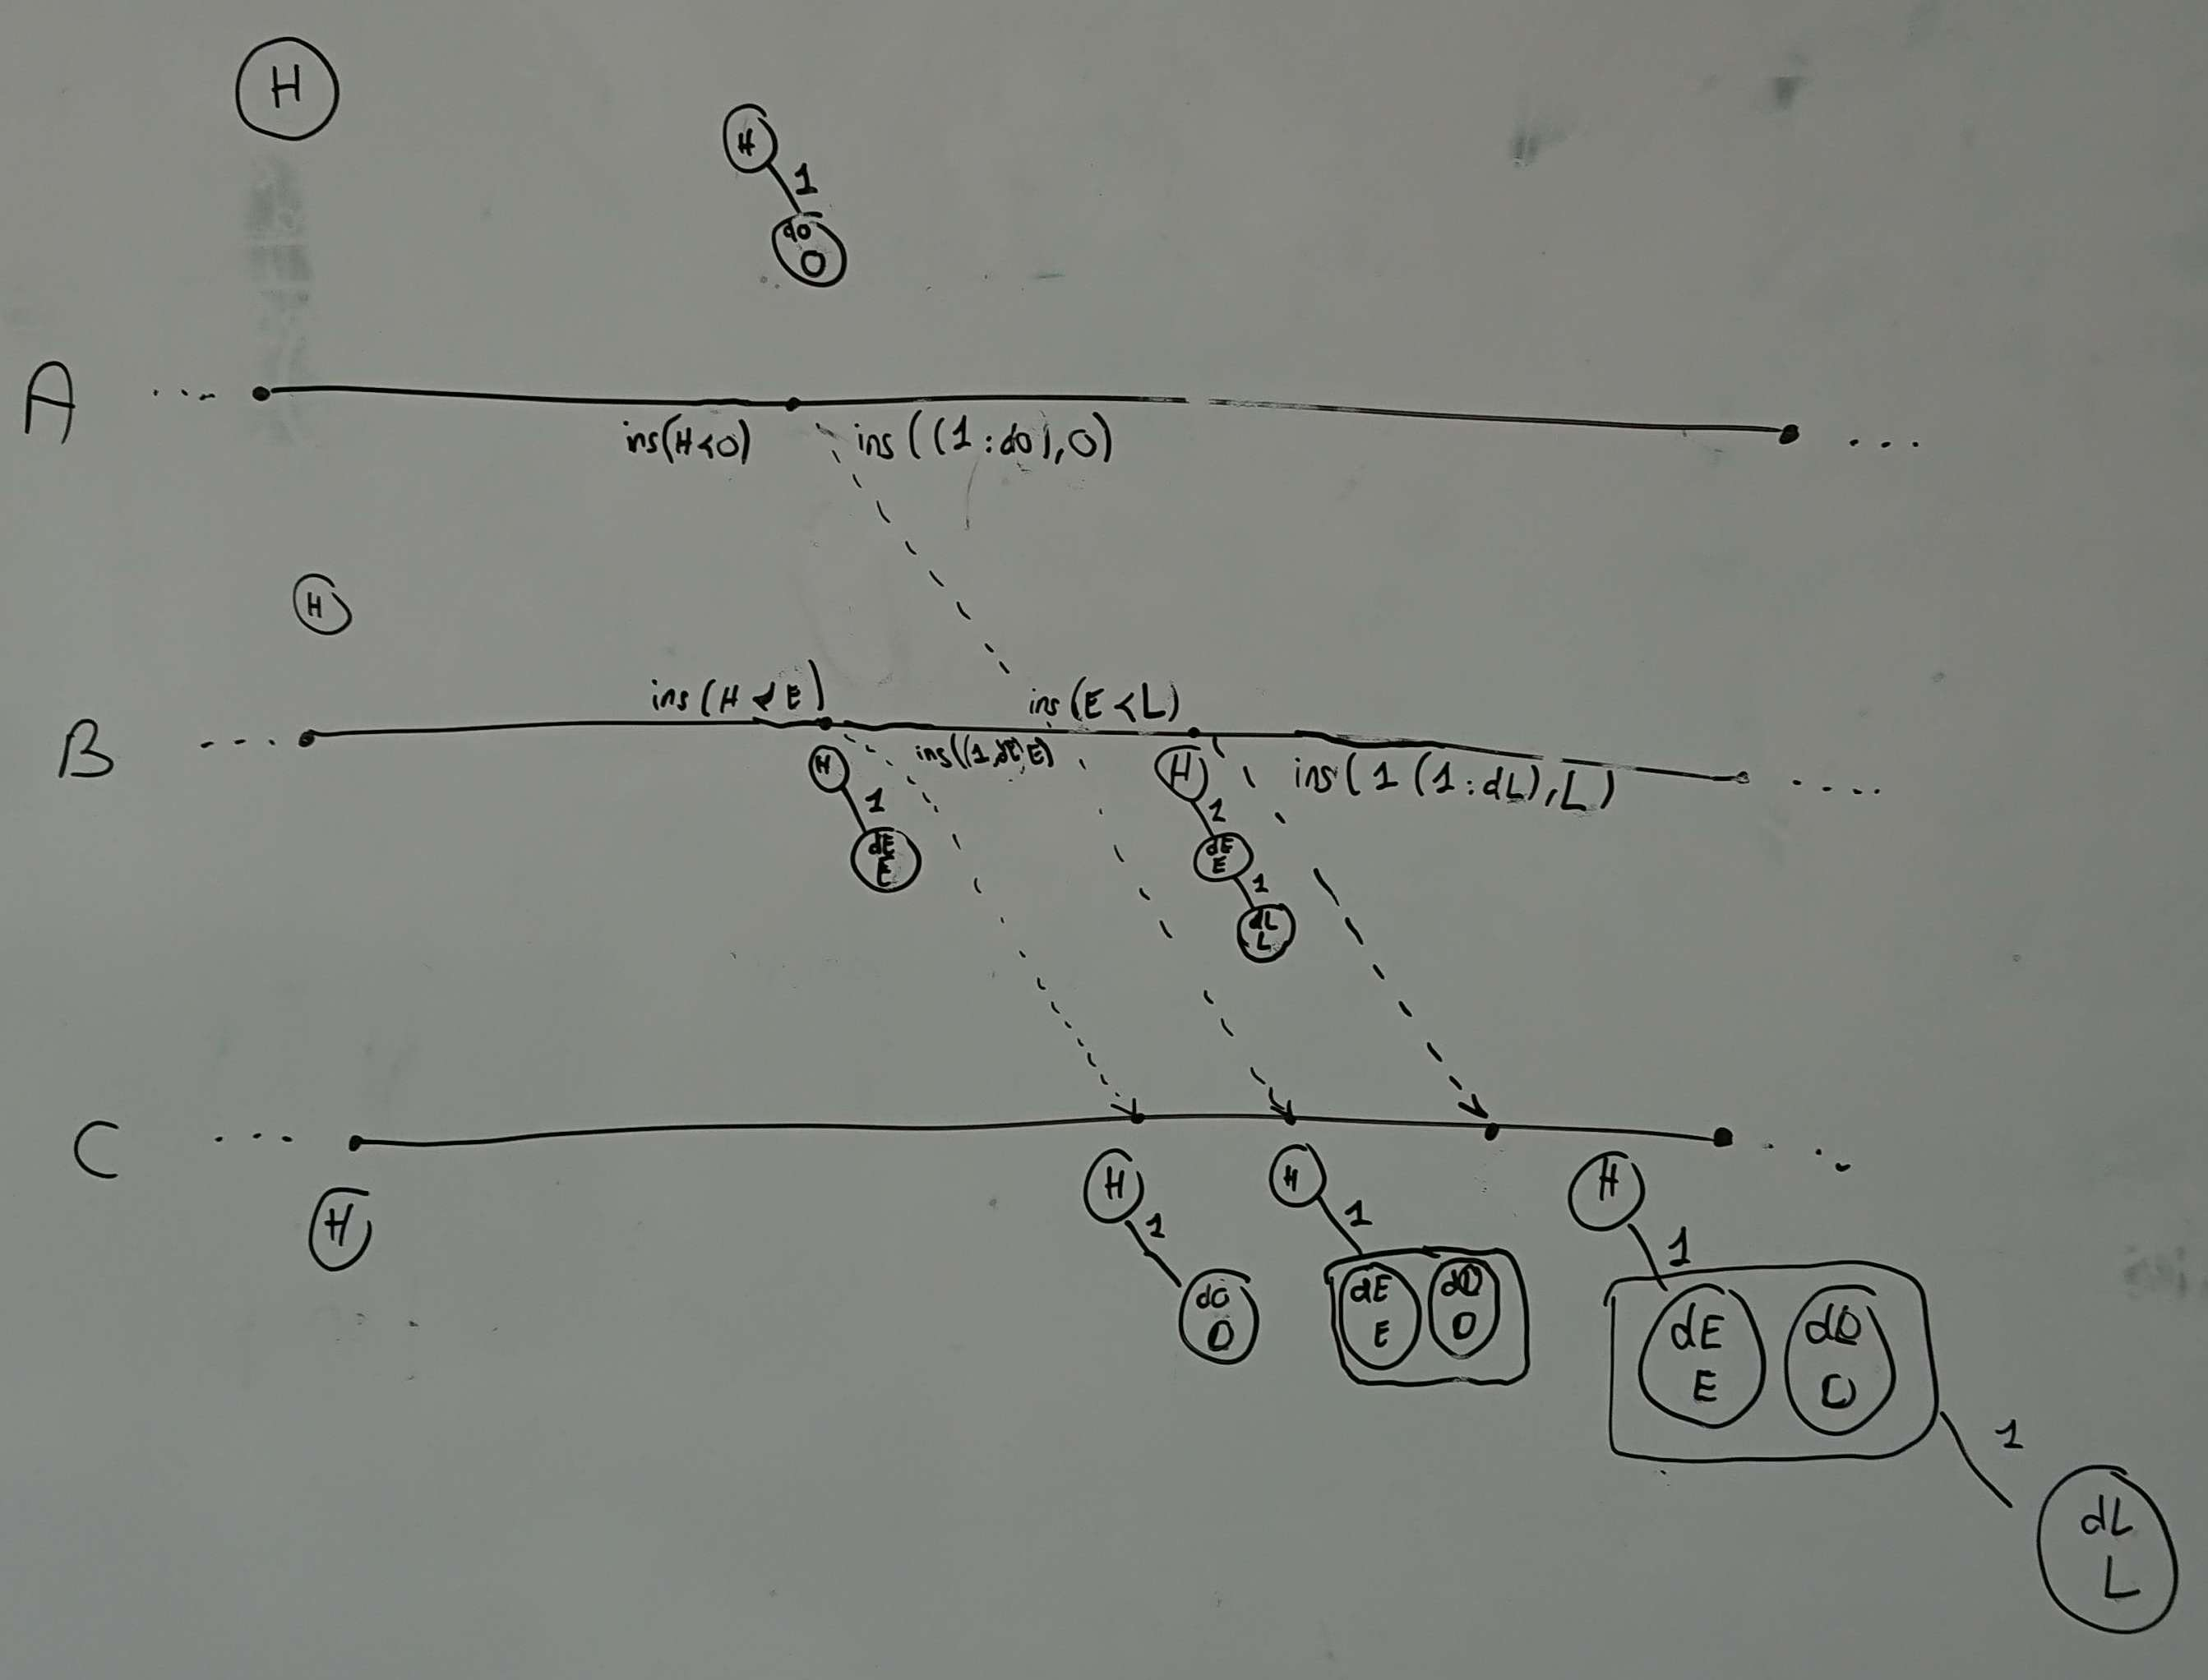
\includegraphics{img/contre-exemple-treedoc}
  }
  \caption{Modifications concurrentes d'une séquence Treedoc résultant en un entrelacement}
\end{figure}

\mnnote{
  TODO: Réaliser au propre contre-exemple.
  Nécessite que $d_E < d_O$, inverser A et B histoire d'éviter toute confusion.
  En soi, C pas nécessaire, à voir si le conserve.
}

\Annex{Algorithmes \textsc{renameId}}

\label{app:rename-id}

\begin{algorithm}[!ht]
  \footnotesize
  \begin{algorithmic}
      \Function{renIdLessThanFirstId}{id, newFirstId}
      \If{id < newFirstId}
          \State \Return id
      \Else
          \State pos $\gets$ position(newFirstId)
          \State nId $\gets$ nodeId(newFirstId)
          \State nSeq $\gets$ nodeSeq(newFirstId)
          \State predNewFirstId $\gets$ \new~Id(pos, nId, nSeq, -1)
          \\
          \State \Return concat(predNewFirstId, id)
          \EndIf
      \EndFunction
      \\
      \Function{renIdGreaterThanLastId}{id, newLastId}
          \If{id < newLastId}
              \State \Return concat(newLastId, id)
          \Else
              \State \Return id
          \EndIf
      \EndFunction
  \end{algorithmic}
  \caption{Remaining functions to rename an identifier}
  \label{alg:appendix-rename-id}
\end{algorithm}

\Annex{Algorithmes \textsc{revertRenameId}}

\label{app:revert-rename-id}

\begin{algorithm}[!ht]
  \footnotesize
  \begin{algorithmic}
      \Function{revRenIdLessThanNewFirstId}{id, firstId, newFirstId}
          \State predNewFirstId $\gets$ createIdFromBase(newFirstId, -1)
          \If{isPrefix(predNewFirstId, id)}
              \State tail $\gets$ getTail(id, 1)
              \If{tail < firstId}
                  \State \Return tail
              \Else
                  \State \Comment{$id$ has been inserted causally after the \emph{rename} op}
                  \State offset $\gets$ getLastOffset(firstId)
                  \State predFirstId $\gets$ createIdFromBase(firstId, offset)
                  \State \Return concat(predFirstId, MAX\_TUPLE, tail)
              \EndIf
          \Else
              \State \Return id
          \EndIf
      \EndFunction
      \\
      \Function{revRenIdGreaterThanNewLastId}{id, lastId}
          \If{id < lastId}
              \State \Comment{$id$ has been inserted causally after the \emph{rename} op}
              \State \Return concat(lastId, MIN\_TUPLE, id)
          \ElsIf{isPrefix(newLastId, id)}
              \State tail $\gets$ getTail(id, 1)
              \If{tail < lastId}
                  \State \Comment{$id$ has been inserted causally after the \emph{rename} op}
                  \State \Return concat(lastId, MIN\_TUPLE, tail)
              \ElsIf{tail < newLastId}
                  \State \Return tail
              \Else
                  \State \Comment{$id$ has been inserted causally after the \emph{rename} op}
                  \State \Return id
              \EndIf
          \Else
              \State \Return id
          \EndIf
      \EndFunction
  \end{algorithmic}
  \caption{Remaining functions to revert an identifier renaming}
  \label{alg:appendix-revert-rename-id}
\end{algorithm}

%
%%-------------------------------------------------------------------
%%                         Le glossaire
%%-------------------------------------------------------------------
%\BeginGloWith{Voici un glossaire tout-à-fait fictif,
%              introduit par un texte sur toute la largeur
%              des deux colonnes.}
%\twocolumn
%\PrintGlossary

%-------------------------------------------------------------------
%              L'index (toujours sur deux colonnes)
%-------------------------------------------------------------------
\BeginIndWith{Voici un index}
\PrintIndex

\onecolumn

%-------------------------------------------------------------------
%                       La bibliographie
%-------------------------------------------------------------------

% La bibliographie (comme d'habitude)

%\nocite{*}
%\bibliographystyle{named}

\printbibliography

%-------------------------------------------------------------------
%                          Les résumés
%-------------------------------------------------------------------
% (si le résumé apparaît sur une colonne étroite, avec la
% bibliographie à gauche, c'est sans doute parce que vous avez
% oublié de générer les fichiers d'index et de glossaire...)

\NumberAbstractPages
\begin{ThesisAbstract}
  \begin{FrenchAbstract}
    Afin d'assurer leur haute disponibilité, les systèmes distribués à large échelle se doivent de répliquer leurs données tout en minimisant les coordinations nécessaires entre noeuds.
    Pour concevoir de tels systèmes, la littérature et l'industrie adoptent de plus en plus l'utilisation de types de données répliquées sans conflits (CRDTs).
    Les CRDTs sont des types de données qui offrent des comportements similaires aux types existants, tel l'Ensemble ou la Séquence.
    Ils se distinguent cependant des types traditionnels par leur spécification, qui supporte nativement les modifications concurrentes.
    À cette fin, les CRDTs incorporent un mécanisme de résolution de conflits au sein de leur spécification.

    Afin de résoudre les conflits de manière déterministe, les CRDTs associent généralement des identifiants aux éléments stockés au sein de la structure de données.
    Les identifiants doivent respecter un ensemble de contraintes en fonction du CRDT, telles que l'unicité ou l'appartenance à un ordre dense.
    Ces contraintes empêchent de borner la taille des identifiants.
    La taille des identifiants utilisés croît alors continuellement avec le nombre de modifications effectuées, aggravant le surcoût lié à l'utilisation des CRDTs par rapport aux structures de données traditionnelles.
    Le but de cette thèse est de proposer des solutions pour pallier ce problème.

    Nous présentons dans cette thèse deux contributions visant à répondre à ce problème :
    \begin{enumerate*}
      \item Un nouveau CRDT pour Séquence, RenamableLogootSplit, qui intègre un mécanisme de renommage à sa spécification.
      Ce mécanisme de renommage permet aux noeuds du système de réattribuer des identifiants de taille minimale aux éléments de la séquence.
      Cependant, cette première version requiert une coordination entre les noeuds pour effectuer un renommage.
      L'évaluation expérimentale montre que le mécanisme de renommage permet de réinitialiser à chaque renommage le surcoût lié à l'utilisation du CRDT.
      \item Une seconde version de RenamableLogootSplit conçue pour une utilisation dans un système distribué.
      Cette nouvelle version permet aux noeuds de déclencher un renommage sans coordination préalable.
      L'évaluation expérimentale montre que cette nouvelle version présente un surcoût temporaire en cas de renommages concurrents, mais que ce surcoût est à terme.
    \end{enumerate*}
    \KeyWords{CRDTs, édition collaborative en temps réel, cohérence à terme, optimisation mémoire, performance}
  \end{FrenchAbstract}
  \begin{EnglishAbstract}
    \KeyWords{CRDTs, real-time collaborative editing, eventual consistency, memory-wise optimisation, performance}
  \end{EnglishAbstract}
\end{ThesisAbstract}


\end{document}



